\chapter{Glossary}
\noindent\textbf{Quantum Artefact} is the general term used for a solution to a problem using quantum computation.
Quantum algorithms and quantum circuits are both types of quantum artefacts.

\noindent\textbf{Quantum Circuit} is an ordered sequence of quantum gate that affects a fixed number of qubits.

\noindent\textbf{Quantum Algorithm} is an ordered sequence of instructions that when followed create a quantum circuit.
The instructions can use variables such as the system size resulting in different circuits for different values.

\noindent\textbf{Quantum Gate} is a physical implementation that performs a specific unitary operation.

\noindent\textbf{Unitary Operation} is an operation that when its defining matrix is multiplied by its complex conjugate the result is the identity.

\noindent\textbf{System Size} is the number of qubits that a quantum circuit affects.

\noindent\textbf{Ket} represents a basis function of the respective Hilbert Space, $\mathcal{H}$, as a column vector.

\noindent\textbf{Bra} denote the 'dual vector' of the corresponding Ket.

% \noindent\textbf{Hilbert Space} extend the simple Euclidean vector space into a potentially infinite dimension function space.

\noindent\textbf{Hermitian Conjugate} is the matrix produced when each element in the matrix U is replaced by its complex conjugate and then the resulting matrix is transposed.

\chapter{User Guide}
\label{sec:userguide}

This appendix is a walk through of how to use the framework and the provided client to search for a quantum algorithm to solve the Max Problem.
This is a simple permutation problem.
The goal is to take a permutation of the values $0\rightarrow3$ and return the index of the maximum value, $3$.

This is used as an experiment in Massey's thesis\cite{masseythesis} for the Q-Pace III system.
The Q-Pace III was able to produce a probabilistic solution to the problem.

There are 24, $4!$, permutation functions possible.
To encode the four values requires four qubits.
This is done using superposition.

The permutation $(0,1,2,3)\rightarrow(w,x,y,z)$ is encoded as the superposition of $\frac{1}{2}(\ket{00w_1w_0}+\ket{01x_1x_0}+\ket{10y_1y_0}+\ket{11z_0z_1})$.
There are several options when selecting the encoding of the expected output of the system.
This is due to the output being two qubits, as it is an index between $0$ and $3$, but the input requires four qubits.
Three of the encoding choices are $\ket{**a_1a_0}$, $\ket{a_1a_0**}$ and $\ket{a_1a_0a_1a_0}$, where$*$ denotes that we don't care what the value is.
The encoding that we shall use in the walk through is $\ket{a_1a_0**}$ so that it is only the highest significant qubits that we are actually interested in.
% This is to try and help the search by increasing the number of final states that the circuit can produce and be considered successful.

Figure \ref{fig:maxprobtcs} shows the list of all $24$ test cases.

\begin{figure}
\begin{center}
 \begin{tabular}{c|ccc|} 
 Test Case ID & Input State& $\rightarrow$ & Output State \\  \hline
  1 & $\frac{1}{2}(\ket{0000}+\ket{0101}+\ket{1010}+\ket{1111})$ & $\rightarrow$ & $\frac{1}{2}(\ket{1100}+\ket{1101}+\ket{1110}+\ket{1111})$ \\ %\hline
  2 & $\frac{1}{2}(\ket{0000}+\ket{0101}+\ket{1011}+\ket{1110})$ & $\rightarrow$ & $\frac{1}{2}(\ket{1000}+\ket{1001}+\ket{1010}+\ket{1011})$ \\ %\hline
  3 & $\frac{1}{2}(\ket{0000}+\ket{0110}+\ket{1001}+\ket{1111})$ & $\rightarrow$ & $\frac{1}{2}(\ket{1100}+\ket{1101}+\ket{1110}+\ket{1111})$ \\ %\hline
  4 & $\frac{1}{2}(\ket{0000}+\ket{0110}+\ket{1011}+\ket{1101})$ & $\rightarrow$ & $\frac{1}{2}(\ket{1000}+\ket{1001}+\ket{1010}+\ket{1011})$ \\ %\hline
  5 & $\frac{1}{2}(\ket{0000}+\ket{0111}+\ket{1001}+\ket{1110})$ & $\rightarrow$ & $\frac{1}{2}(\ket{0100}+\ket{0101}+\ket{0110}+\ket{0111})$ \\ %\hline
  6 & $\frac{1}{2}(\ket{0000}+\ket{0111}+\ket{1010}+\ket{1101})$ & $\rightarrow$ & $\frac{1}{2}(\ket{0100}+\ket{0101}+\ket{0110}+\ket{0111})$ \\ \hline
  7 & $\frac{1}{2}(\ket{0001}+\ket{0100}+\ket{1010}+\ket{1111})$ & $\rightarrow$ & $\frac{1}{2}(\ket{1100}+\ket{1101}+\ket{1110}+\ket{1111})$ \\ %\hline
  8 & $\frac{1}{2}(\ket{0001}+\ket{0100}+\ket{1011}+\ket{1110})$ & $\rightarrow$ & $\frac{1}{2}(\ket{1000}+\ket{1001}+\ket{1010}+\ket{1011})$ \\ %\hline
  9 & $\frac{1}{2}(\ket{0001}+\ket{0110}+\ket{1000}+\ket{1111})$ & $\rightarrow$ & $\frac{1}{2}(\ket{1100}+\ket{1101}+\ket{1101}+\ket{1111})$ \\ %\hline
  10 & $\frac{1}{2}(\ket{0001}+\ket{0110}+\ket{1011}+\ket{1100})$ & $\rightarrow$ & $\frac{1}{2}(\ket{1000}+\ket{1001}+\ket{1010}+\ket{1011})$ \\ %\hline
  11 & $\frac{1}{2}(\ket{0001}+\ket{0111}+\ket{1000}+\ket{1110})$ & $\rightarrow$ & $\frac{1}{2}(\ket{0100}+\ket{0101}+\ket{0110}+\ket{0111})$ \\ %\hline
  12 & $\frac{1}{2}(\ket{0001}+\ket{0111}+\ket{1010}+\ket{1100})$ & $\rightarrow$ & $\frac{1}{2}(\ket{0100}+\ket{0101}+\ket{0110}+\ket{0111})$ \\ \hline
  13 & $\frac{1}{2}(\ket{0010}+\ket{0100}+\ket{1001}+\ket{1111})$ & $\rightarrow$ & $\frac{1}{2}(\ket{1100}+\ket{1101}+\ket{1101}+\ket{1111})$ \\ %\hline
  14 & $\frac{1}{2}(\ket{0010}+\ket{0100}+\ket{1011}+\ket{1101})$ & $\rightarrow$ & $\frac{1}{2}(\ket{1000}+\ket{1001}+\ket{1010}+\ket{1011})$ \\ %\hline
  15 & $\frac{1}{2}(\ket{0010}+\ket{0101}+\ket{1000}+\ket{1111})$ & $\rightarrow$ & $\frac{1}{2}(\ket{1100}+\ket{1101}+\ket{1110}+\ket{1111})$ \\ %\hline
  16 & $\frac{1}{2}(\ket{0010}+\ket{0101}+\ket{1011}+\ket{1100})$ & $\rightarrow$ & $\frac{1}{2}(\ket{1000}+\ket{1001}+\ket{1010}+\ket{1011})$ \\ %\hline
  17 & $\frac{1}{2}(\ket{0010}+\ket{0111}+\ket{1000}+\ket{1101})$ & $\rightarrow$ & $\frac{1}{2}(\ket{0100}+\ket{0101}+\ket{0110}+\ket{0111})$ \\ %\hline
  18 & $\frac{1}{2}(\ket{0010}+\ket{0111}+\ket{1001}+\ket{1100})$ & $\rightarrow$ & $\frac{1}{2}(\ket{0100}+\ket{0101}+\ket{0110}+\ket{0111})$ \\ \hline
  19 & $\frac{1}{2}(\ket{0011}+\ket{0100}+\ket{1001}+\ket{1110})$ & $\rightarrow$ & $\frac{1}{2}(\ket{0000}+\ket{0001}+\ket{0010}+\ket{0011})$ \\ %\hline
  20 & $\frac{1}{2}(\ket{0011}+\ket{0100}+\ket{1010}+\ket{1101})$ & $\rightarrow$ & $\frac{1}{2}(\ket{0000}+\ket{0001}+\ket{0010}+\ket{0011})$ \\ %\hline
  21 & $\frac{1}{2}(\ket{0011}+\ket{0101}+\ket{1000}+\ket{1110})$ & $\rightarrow$ & $\frac{1}{2}(\ket{0000}+\ket{0001}+\ket{0010}+\ket{0011})$ \\ %\hline
  22 & $\frac{1}{2}(\ket{0011}+\ket{0101}+\ket{1010}+\ket{1100})$ & $\rightarrow$ & $\frac{1}{2}(\ket{0000}+\ket{0001}+\ket{0010}+\ket{0011})$ \\ %\hline
  23 & $\frac{1}{2}(\ket{0011}+\ket{0110}+\ket{1000}+\ket{1101})$ & $\rightarrow$ & $\frac{1}{2}(\ket{0000}+\ket{0001}+\ket{0010}+\ket{0011})$ \\ %\hline
  24 & $\frac{1}{2}(\ket{0011}+\ket{0110}+\ket{1001}+\ket{1100})$ & $\rightarrow$ & $\frac{1}{2}(\ket{0000}+\ket{0001}+\ket{0010}+\ket{0011})$ \\ \hline
 \end{tabular}
\end{center}
\caption{Max Problem Test Cases}
\label{fig:maxprobtcs}
\end{figure}

\section{Creating the Search Problem}
\label{sec:createsearchproblem}

Using the test cases listed in Figure \ref{fig:maxprobtcs} this section will go through how to create a search problem for the Max problem.
The walk through will use the provided client rather than the standalone editor but as the two use the same components using the guide with the standalone editor should not cause any problems.
The walk through shall only include the input of two randomly chosen test cases, $1$ and $10$.

\lstset{language=bash,breaklines=true,breakatwhitespace=false,numbers=none}
\begin{enumerate}
 \item Launch the client with the command below
\begin{lstlisting}
java -jar MengQuantum.jar config/SearchEngine.xml config/FitnessFunction.xml config/Problems.xml false
\end{lstlisting}
The client shall launch and you shall be provided with the Graphical User Interface as shown in Figure \ref{fig:walkthrough1}.

\item Using the mouse, left click on the button labelled ``Create'', as shown in Figure \ref{fig:walkthrough2}.
When prompted, select 0 custom gates as none are required for the Max problem.
The ``Create Problem and Test Suite'' dialog box shall be displayed, as shown in Figure \ref{fig:walkthrough3}.

\item Using the mouse, left click in the text area to the right of the ``Name'' and enter ``Max Problem''.

\item Using the mouse, left click on the button labelled ``Select Destination File''.
A new dialog box shall open to select the location and file name for the test suite definition file.
The dialog box is a standard ``file chooser'' as used in many applications so the operation of it should be familiar to all users.

\item Using the file chooser, navigate to the ``Config'' directory provided in the distribution.
A number of XML files should be listed, including SearchEngine.xml and FitnessFunction.xml.
Using the mouse, left click in the text area next to ``File Name:'' and enter ``maxproblem''.
The ``.xml'' is added automatically by the software.
Using the mouse, left click on the button labelled ``Open'' to close the dialog box.

\item Now we can start entering the test cases.
Using the mouse, left click on the button labelled ``Add Test Set'' and, when prompted, enter $4$ as the number of qubits.
This shall change the appearance of the dialog box to match that shown in Figure \ref{fig:walkthrough4}.

\item We shall enter test case $1$.

The input state is shown in the left hand table.
Put the value $0.5$ in the second column of the rows labelled with the states $\ket{0000}$, $\ket{0101}$, $\ket{1010}$ and $\ket{1111})$.

The output state is shown in the right hand table.
Put the value $0.5$ in the second column of the rows labelled with the states $\ket{1100}$, $\ket{1101}$, $\ket{1110}$ and $\ket{1111})$.
The value $0.5$ is used as it means that the probability of any of them is $\frac{1}{4}$ as no specific output is desired as long as the two most significant qubits match.

\item \label{enum:addtcstep} Using the mouse, left click on the button labelled ``Add Test Case''.
We shall now enter test case $10$.

The input state is shown in the left hand table.
Put the value $0.5$ in the second column of the rows labelled with the states $\ket{0001}$, $\ket{0100}$, $\ket{1010}$ and $\ket{1111})$.

The output state is shown in the right hand table.
Put the value $0.5$ in the second column of the rows labelled with the states $\ket{1000}$, $\ket{1001}$, $\ket{1010}$ and $\ket{1011})$.

\item Using the mouse, left click in the text area to the right of the ``Description'' label and enter ``Max Problem as described by Massey''.

\item Using the mouse, left click on the button labelled ``Okay'' to save the test suite to file and close the dialog box.

\item \label{enum:createsaveprobs}Optional: To ensure that the ``Max Problem'' search problem is registered and loaded when the client is launched in the future left click on the button labelled ``Save''.
This ``Save'' button does not save the test suite, this is done automatically by the ``Create Problem'' dialog box.
It saves the changes to the ``config/Problems.xml'' file containing the problem definitions, see Section \ref{sec:problemman}.
\end{enumerate}

The steps outlined produce a very simple test suite for the search to use.
Providing the search with more of the $24$ test cases that are available than the two created by the steps above is likely to improve the performance of the search.
To create additional test cases repeat step \ref{enum:addtcstep} for each additional test case desired.

\section{Loading a Predefined Search Problem}
This section shall provide a guide to creating a search problem by using an existing test suite definition XML file.
The example that shall be used is if the user followed the walk through in Section \ref{sec:createsearchproblem} by did not perform Step \ref{enum:createsaveprobs}.
This would result in the ``Max Problem'' created not to be registered, and therefore not listed in the search problem drop down list, once the software is restarted.
This is the process that would have to be performed if a researcher were to try use a test suite created and distribute by another researcher.

\begin{enumerate}
 \item Launch the client with the command below
\begin{lstlisting}
java -jar MengQuantum.jar config/SearchEngine.xml config/FitnessFunction.xml config/Problems.xml false
\end{lstlisting}
The client shall launch and you shall be provided with the Graphical User Interface as shown in Figure \ref{fig:walkthrough1}.

\item Using the mouse, left click on the button labelled Load'', as shown in Figure \ref{fig:walkthrough2}.
The ``Load Test Suite to Create Problem'' dialog box shall be displayed, as shown in Figure \ref{fig:walkthrough5}.

\item Using the mouse, left click in the text area to the right of the ``Name'' and enter ``Max Problem''.

\item Using the mouse, left click on the button labelled ``Select Definition File''.
A new dialog box shall open to select the location and file name for the test suite definition file.
The dialog box is a standard ``file chooser'' as used in many applications so the operation of it should be familiar to all users.

\item Using the file chooser, navigate to the ``Config'' directory provided in the distribution.
A number of XML files should be listed, including SearchEngine.xml and FitnessFunction.xml.
Using the mouse, select the ``maxproblem.xml'' file and left click on the button labelled ``Open'' to close the dialog box.

\item Using the mouse, left click in the text area to the right of the ``Description'' label and enter ``Max Problem as described by Massey''.

\item Using the mouse, left click on the button labelled ``Okay'' to save the test suite to file and close the dialog box.

\item \label{enum:loadsaveprobs}Optional: To ensure that the ``Max Problem'' search problem is registered and loaded when the client is launched in the future left click on the button labelled ``Save''.
It saves the changes to the ``config/Problems.xml'' file containing the problem definitions, see Section \ref{sec:problemman}.

\end{enumerate}

\section{Editing an Existing Search Problem}

Using the test cases listed in Figure \ref{fig:maxprobtcs} this section will go through how to edit the search problem for the Max problem created in Section \ref{sec:createsearchproblem}.
The walk through will use the provided client rather than the standalone editor but as the two use the same components using the guide with the standalone editor should not cause any problems.
With the standalone editor the test suite definition XML file needs to be manually loaded using the ``Open File'' button.
The walk through shall add an additional test case, test case $2$.

\begin{enumerate}
 \item Launch the client with the command below
\begin{lstlisting}
java -jar MengQuantum.jar config/SearchEngine.xml config/FitnessFunction.xml config/Problems.xml false
\end{lstlisting}
The client shall launch and you shall be provided with the Graphical User Interface as shown in Figure \ref{fig:walkthrough1}.

\item Using the problem selection drop down list, select ``Max Problem''.

\item Using the mouse, left click on the button labelled ``Edit Selected Problem'', as shown in Figure \ref{fig:walkthrough2}.
This shall launch the ``Edit Current Problem and Test Suite'' dialog box, as shown in Figure \ref{fig:walkthrough6}.
This dialog box is almost identical to the ``Create Problem and Test Suite'' used in Section \ref{sec:createsearchproblem}.

\item Using the mouse, left click on the button labelled ``Add Test Case''.
We shall now enter test case $2$.

The input state is shown in the left hand table.
Put the value $0.5$ in the second column of the rows labelled with the states $\ket{0000}$, $\ket{0101}$, $\ket{1011}$ and $\ket{1110})$.

The output state is shown in the right hand table.
Put the value $0.5$ in the second column of the rows labelled with the states $\ket{0010}$, $\ket{0110}$, $\ket{1010}$ and $\ket{1110})$.

\item Using the mouse, left click on the button labelled ``Okay''.
A warning dialog box is produced, see Figure \ref{fig:walkthrough7} .
This shows the difference between the ``Edit Current Problem and Test Suite'' dialog box and the ``Create Problem and Test Suite'' used in Section \ref{sec:createsearchproblem}.
When the ``Okay'' button is pressed on the ``Create Problem and Test Suite'' used in Section \ref{sec:createsearchproblem} the test suite definition file is automatically updated.
This is because the ``Create Problem and Test Suite'' creates and entirely new search problem and test suite.
The``Edit Current Problem and Test Suite'' dialog box is used to edit an existing search problem with a pre-existing test suite XML definition file.
A researcher may want to make changes to a search problem for experimentation but not necessarily effect the contents of the test suite XML definition file.

If the researcher does want the test suite XML definition file to be updated to reflect the changes made to the test suite, the button labelled ``Save and Close'' should be used instead of the button labelled ``Okay''.

\end{enumerate}

\section{Carrying Out The Search}
\label{sec:carryingoutthesearch}

This section shall use the search problem created in Section \ref{sec:createsearchproblem} to perform a search.
The search engine that shall be used is the local version of the ``Q-Pace IV Based Search Engine'', see Section \ref{sec:provsearcheng} with the ``Simple'' suitability measure, see Section \ref{sec:simplsuitmeas}.

\begin{enumerate}
 \item Launch the client with the command below
\begin{lstlisting}
java -jar MengQuantum.jar config/SearchEngine.xml config/FitnessFunction.xml config/Problems.xml false
\end{lstlisting}
The client shall launch and you shall be provided with the Graphical User Interface as shown in Figure \ref{fig:walkthrough1}.

\item Using the search engine selection drop down list, select ``Genetic Programming - QPace Local''.

\item Using the suitability selection drop down list, select ``Simple Suitability''.

\item Using the problem selection drop down list, select ``Max Problem''.

\item Using the mouse, left click on the button labelled ``Evolve'', as shown in Figure \ref{fig:walkthrough2}.
This shall open up a new dialog box specific for the search engine selected.

\item \label{enum:searchsettings} Most default settings shall be maintained.
The three items that shall be changed are the number of generations, the mutation rate and the number of search iterations.
Using the mouse, left click in the text area to the right of the ``Generations'' label and enter $2000$.
Using the mouse, left click in the text area to the right of the ``Mutation Rate'' label and enter $0.3$.
Using the mouse, left click in the text area to the right of the ``Number of Iterations'' label and enter $3$.

\item To start the search, click on the button labelled ``Evolve Now''.
This shall initiate the search and the dialog box shall close.
All the selection drop down lists will be disabled so that changes cannot be made during a search.
During the search, a statistics panel is provided as can be see in Figure \ref{fig:walkthrough8}.
If the JPPF version of the search engine were selected,  the statistics panel would provide much less information due to the amount of information available due to the distribution.

\item When the search is complete, the results shall be displayed in the central panel as can be seen in Figure \ref{fig:walkthrough9}.

\end{enumerate}

\section{Analysing the Search Results}

Once the search is completed, the results are shown in the central panel as can be seen in Figure \ref{fig:walkthrough9}.
This section assumes that the results are produced by following the steps in Section \ref{sec:carryingoutthesearch}.

\subsection{Which Search Result?}

In Step \ref{sec:carryingoutthesearch} of Section \ref{sec:carryingoutthesearch} the number of search iterations is set to 3.
This means that three completely separate searches are carried out.
Obviously this means that there are three separate search results produced.
All search results are available for the user to analyse.

The user interface provides a drop down list of all the available search results.
Below the drop down list are the details of the selected results.

\clearpage
\section{Referenced Figures}
\begin{figure}[h!]
  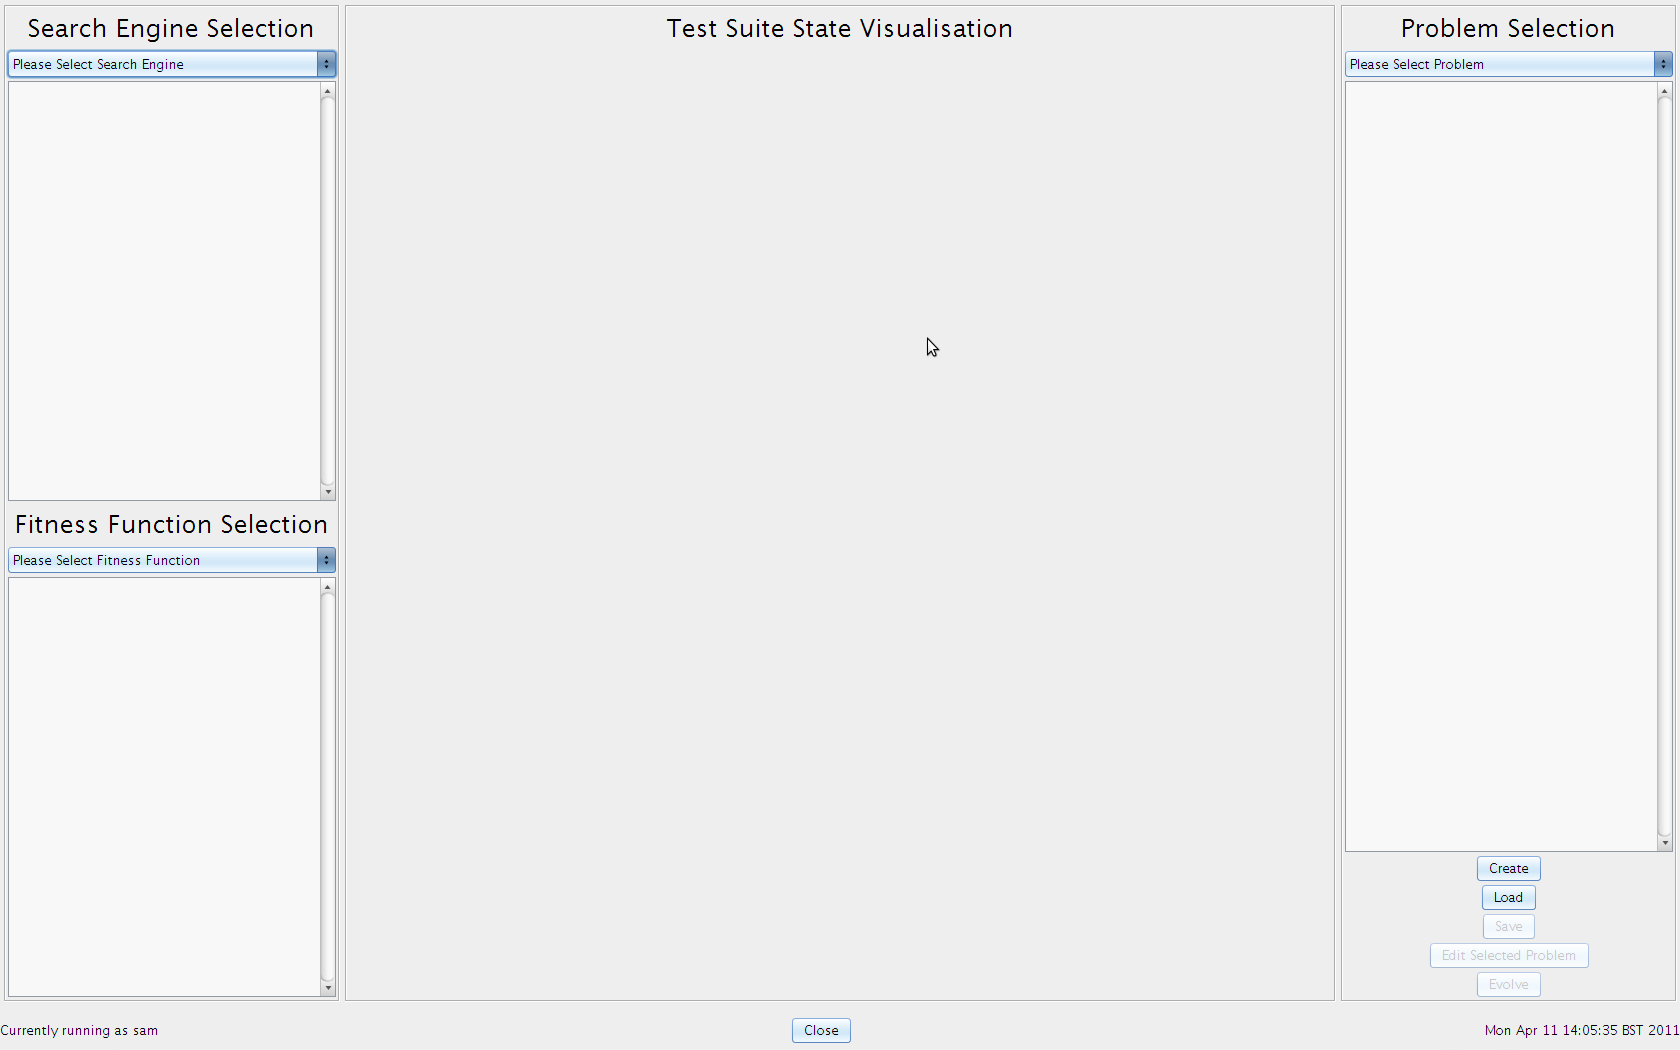
\includegraphics[width=\textwidth]{walkthrough1.png}
 \caption{Initial State of the Client GUI}
 \label{fig:walkthrough1}
\end{figure}

\begin{figure}
\begin{center}
  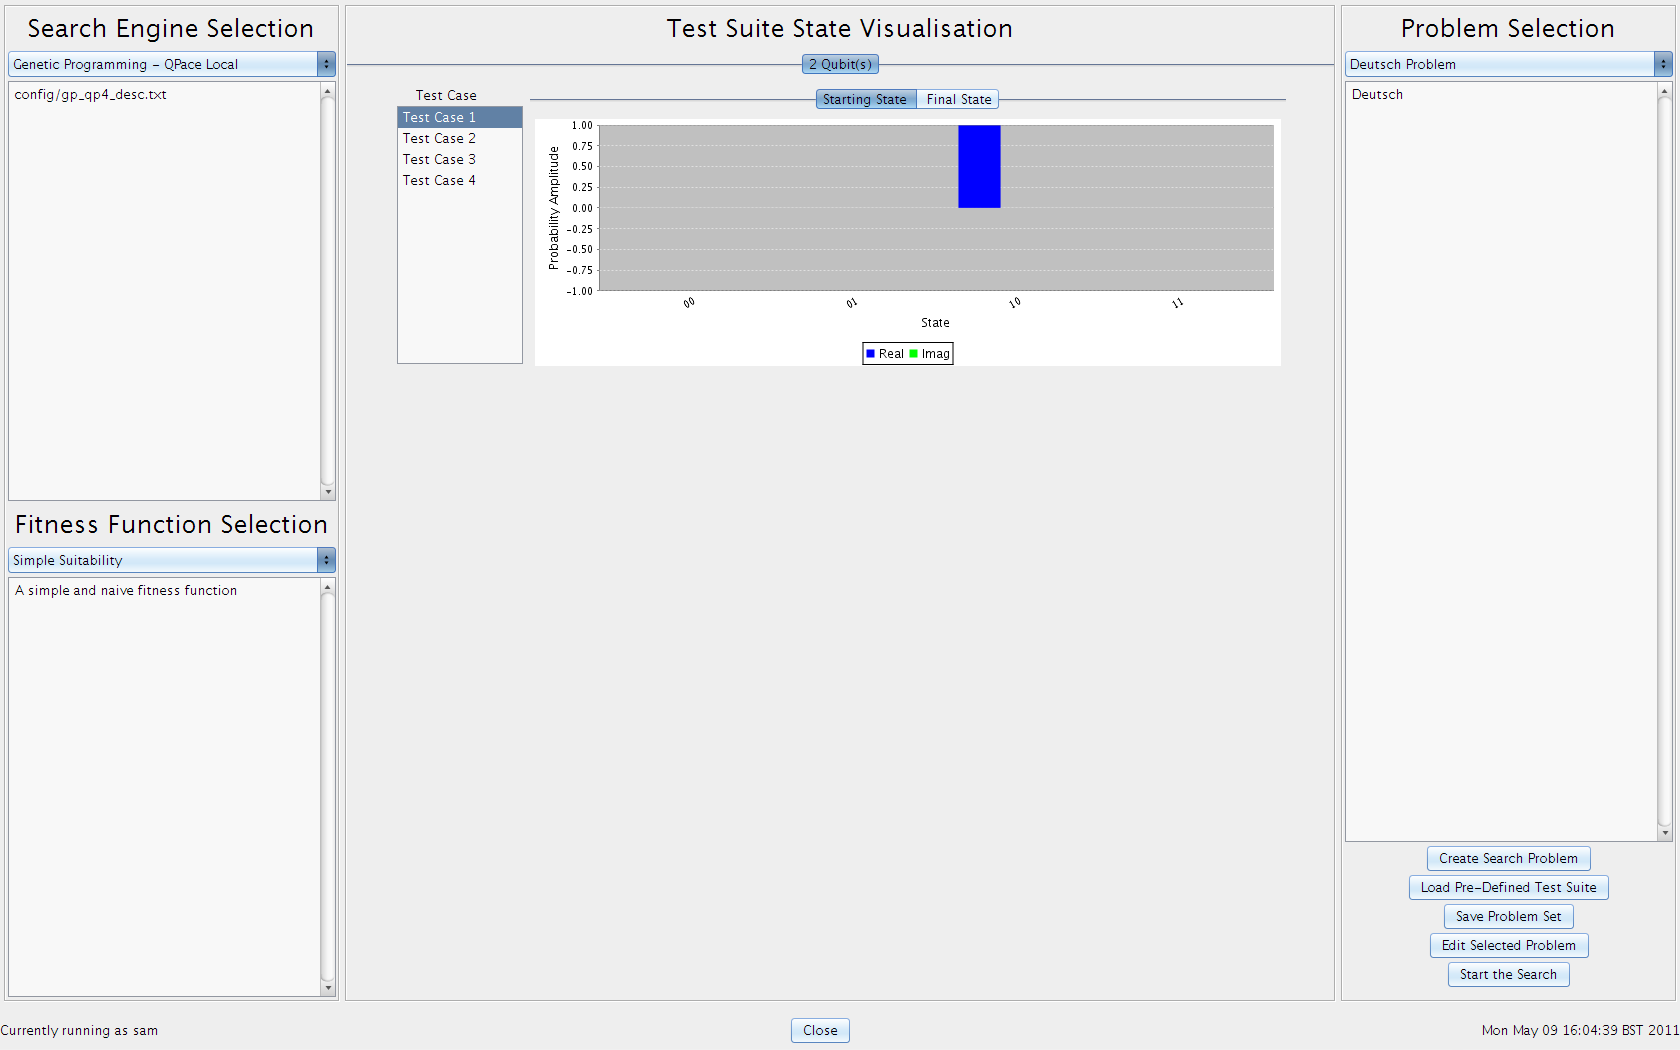
\includegraphics[width=10cm]{walkthrough2.png}
\end{center}
 \caption{Right hand menu}
 \label{fig:walkthrough2}
\end{figure}

\begin{figure}
  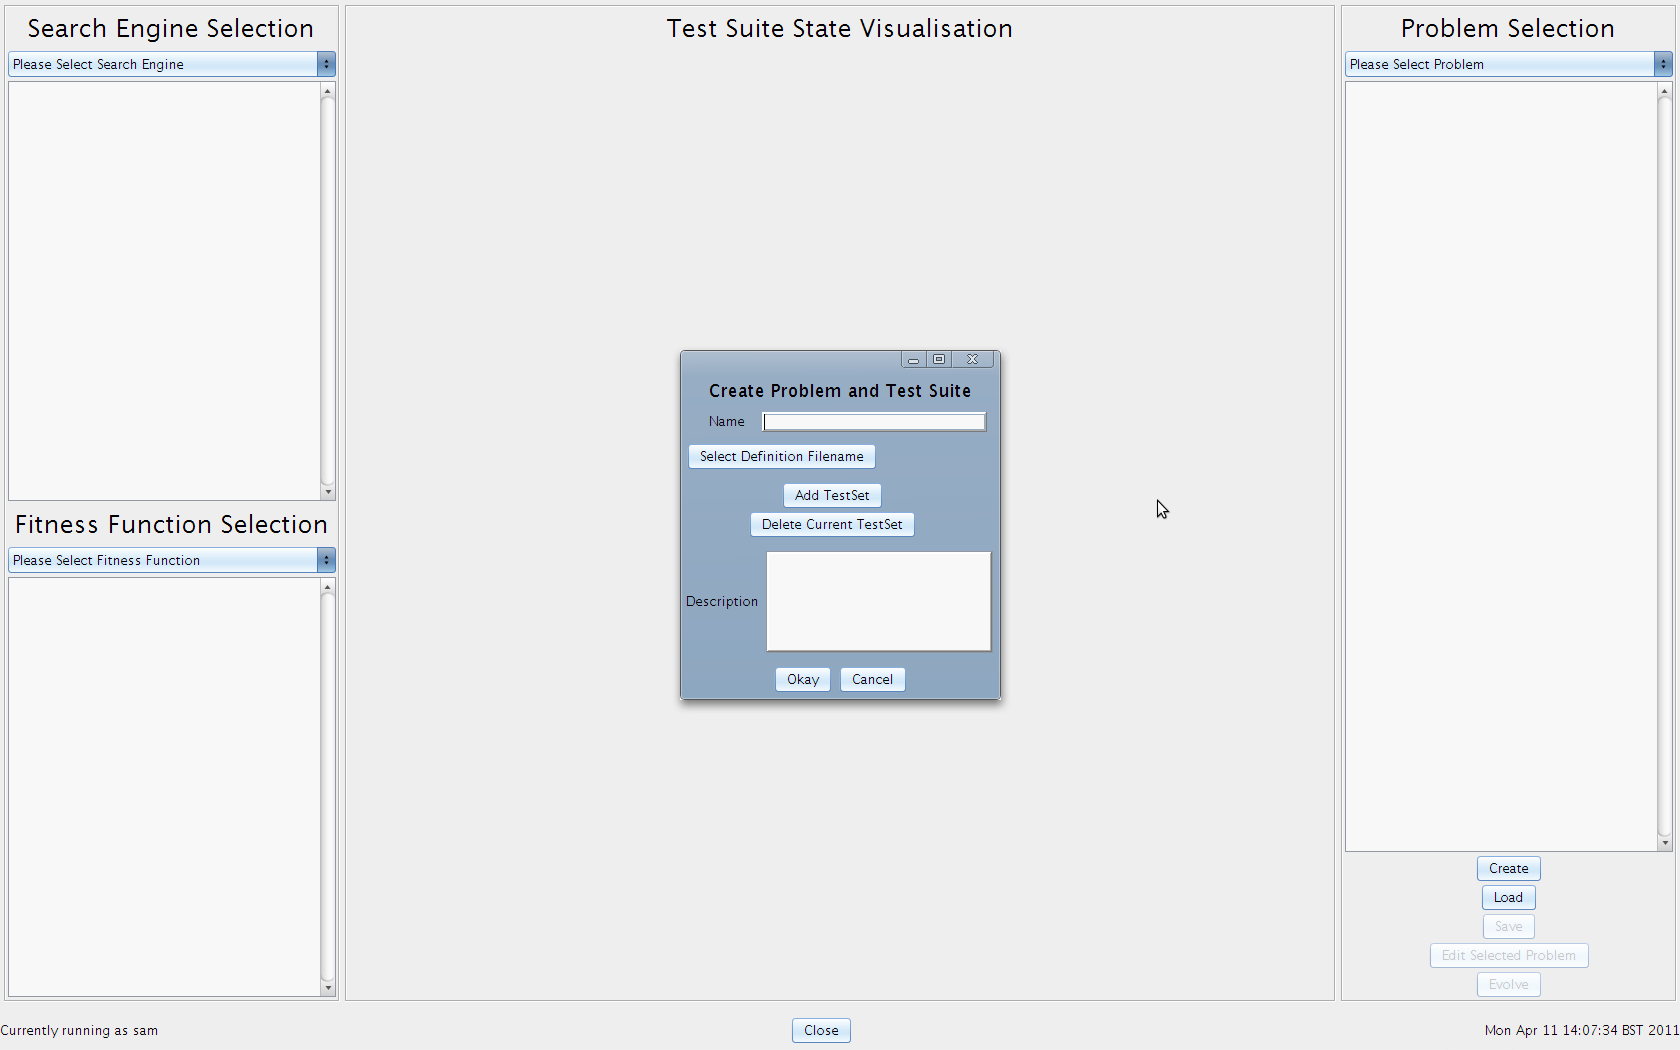
\includegraphics[width=\textwidth]{walkthrough3.png}
 \caption{Create Problem and Test Suite dialog box}
 \label{fig:walkthrough3}
\end{figure}

\begin{figure}
  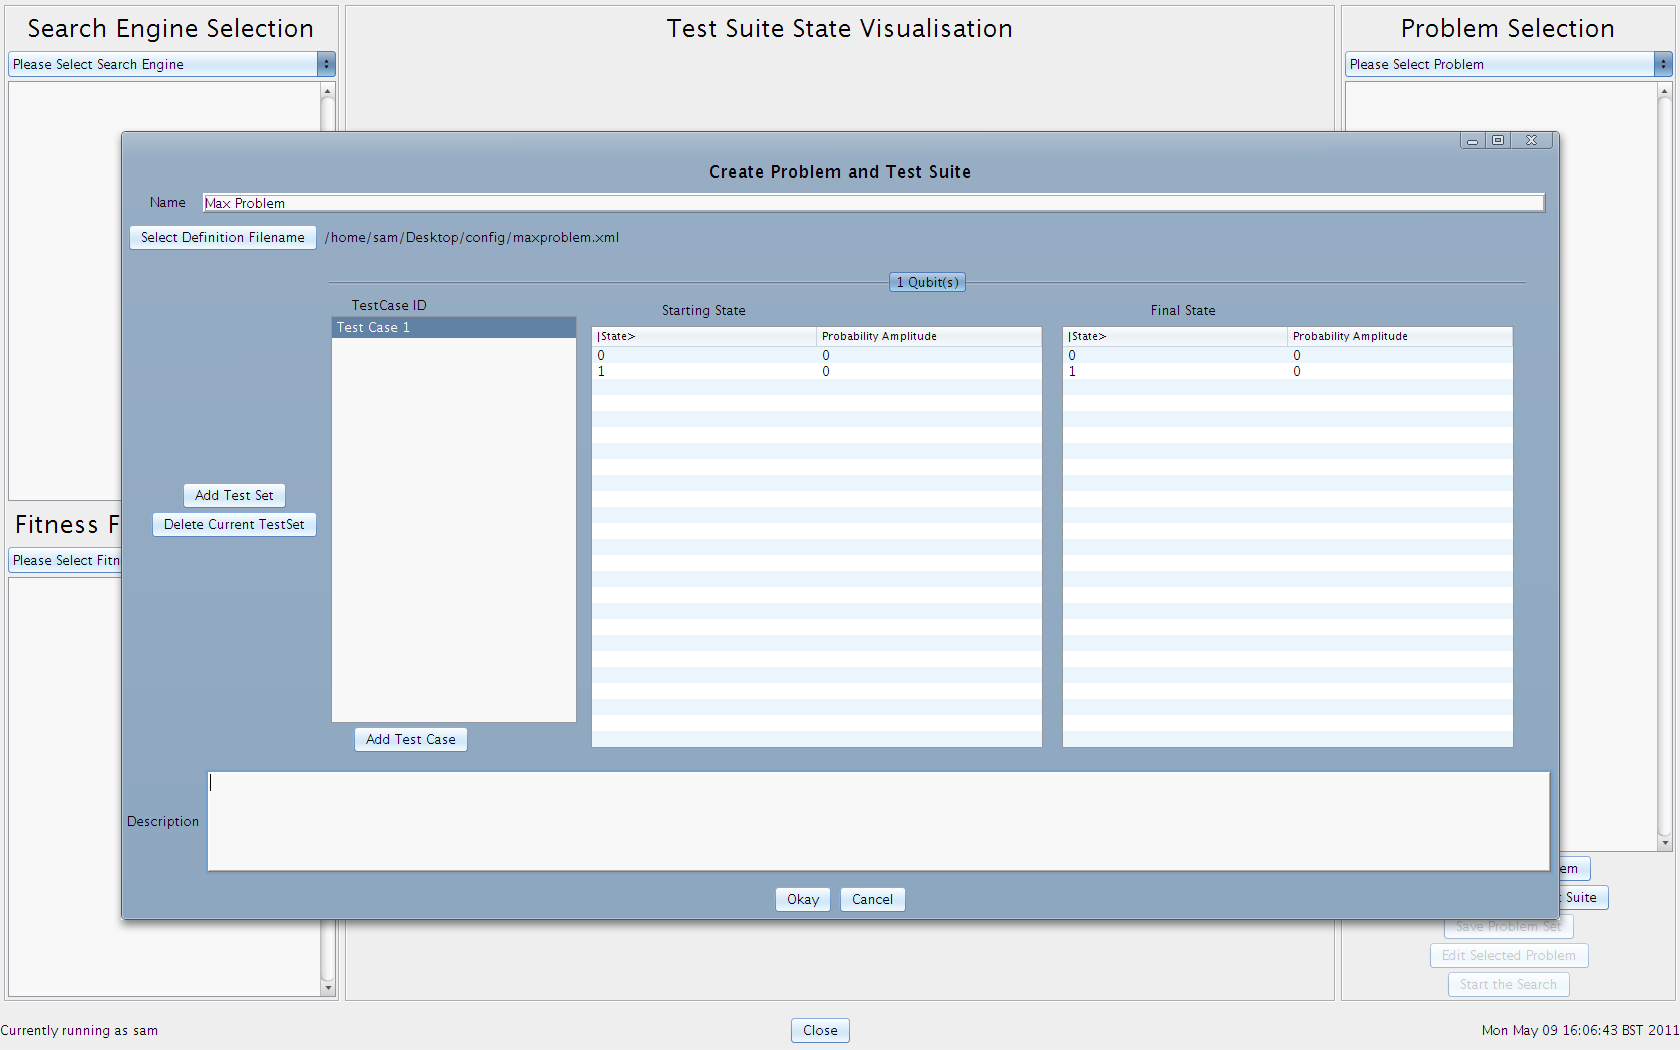
\includegraphics[width=\textwidth]{walkthrough4.png}
 \caption{Full Create Problem and Test Suite dialog box}
 \label{fig:walkthrough4}
\end{figure}

\begin{figure}
  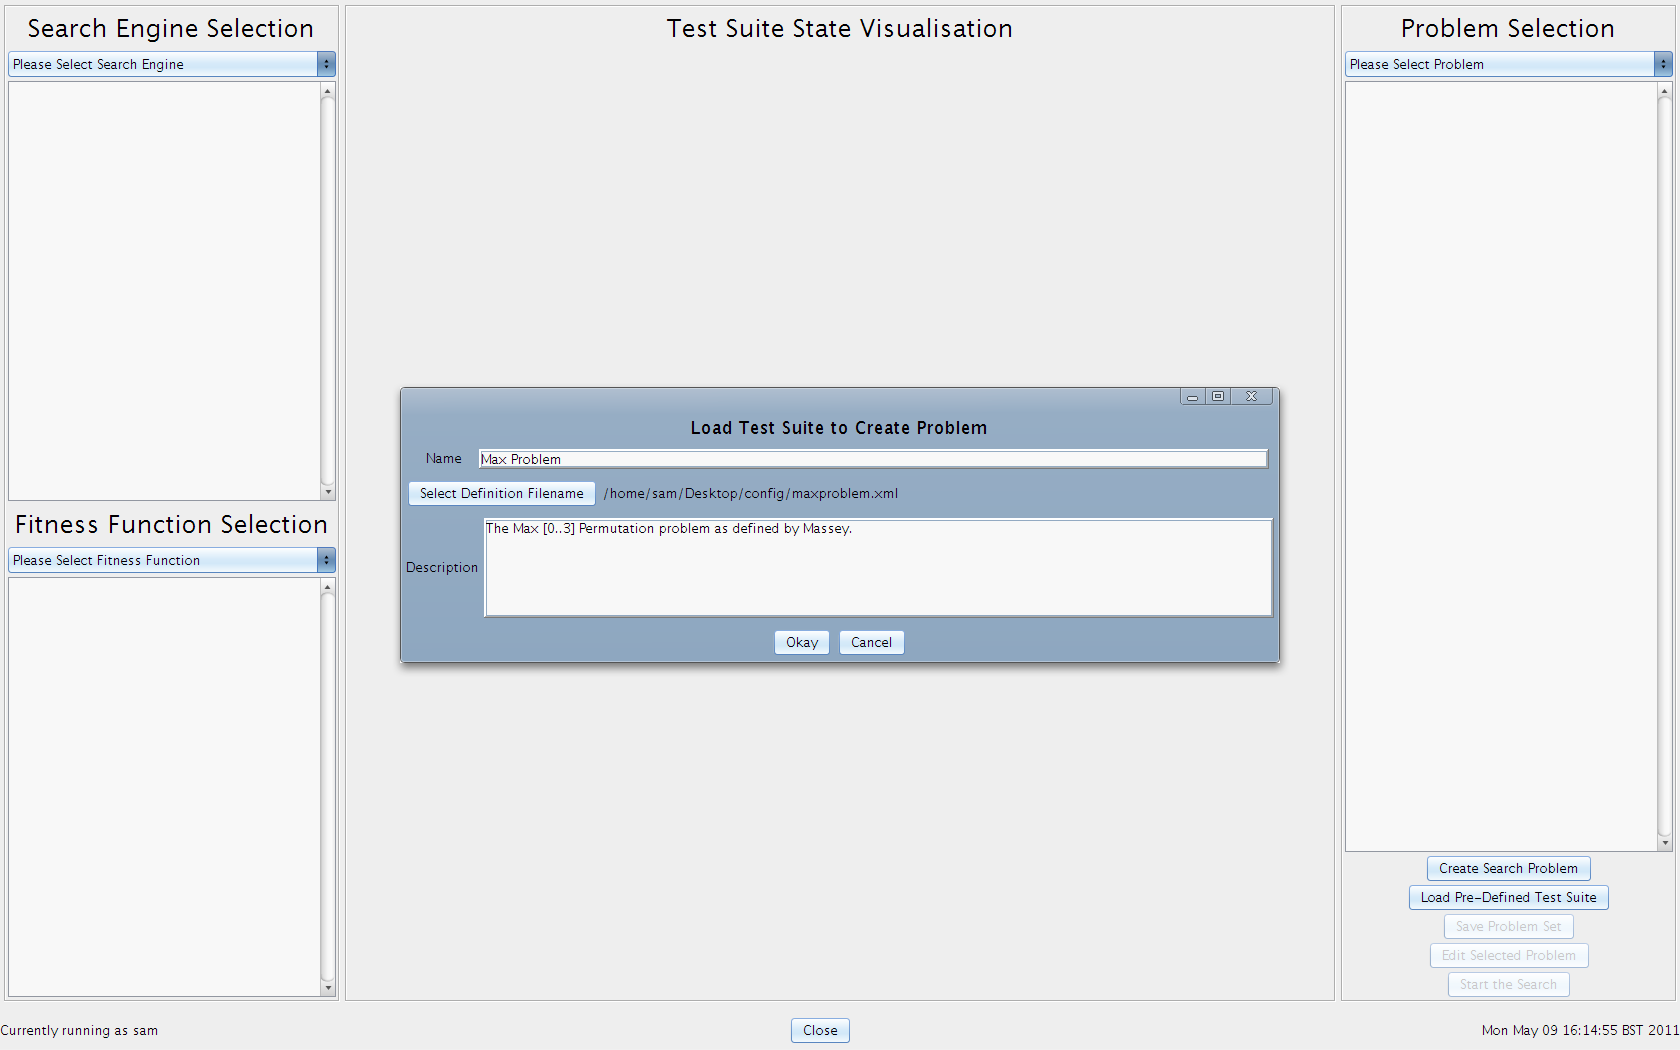
\includegraphics[width=\textwidth]{walkthrough5.png}
 \caption{Load Test Suite to Create Problem dialog box}
 \label{fig:walkthrough5}
\end{figure}

\begin{figure}
  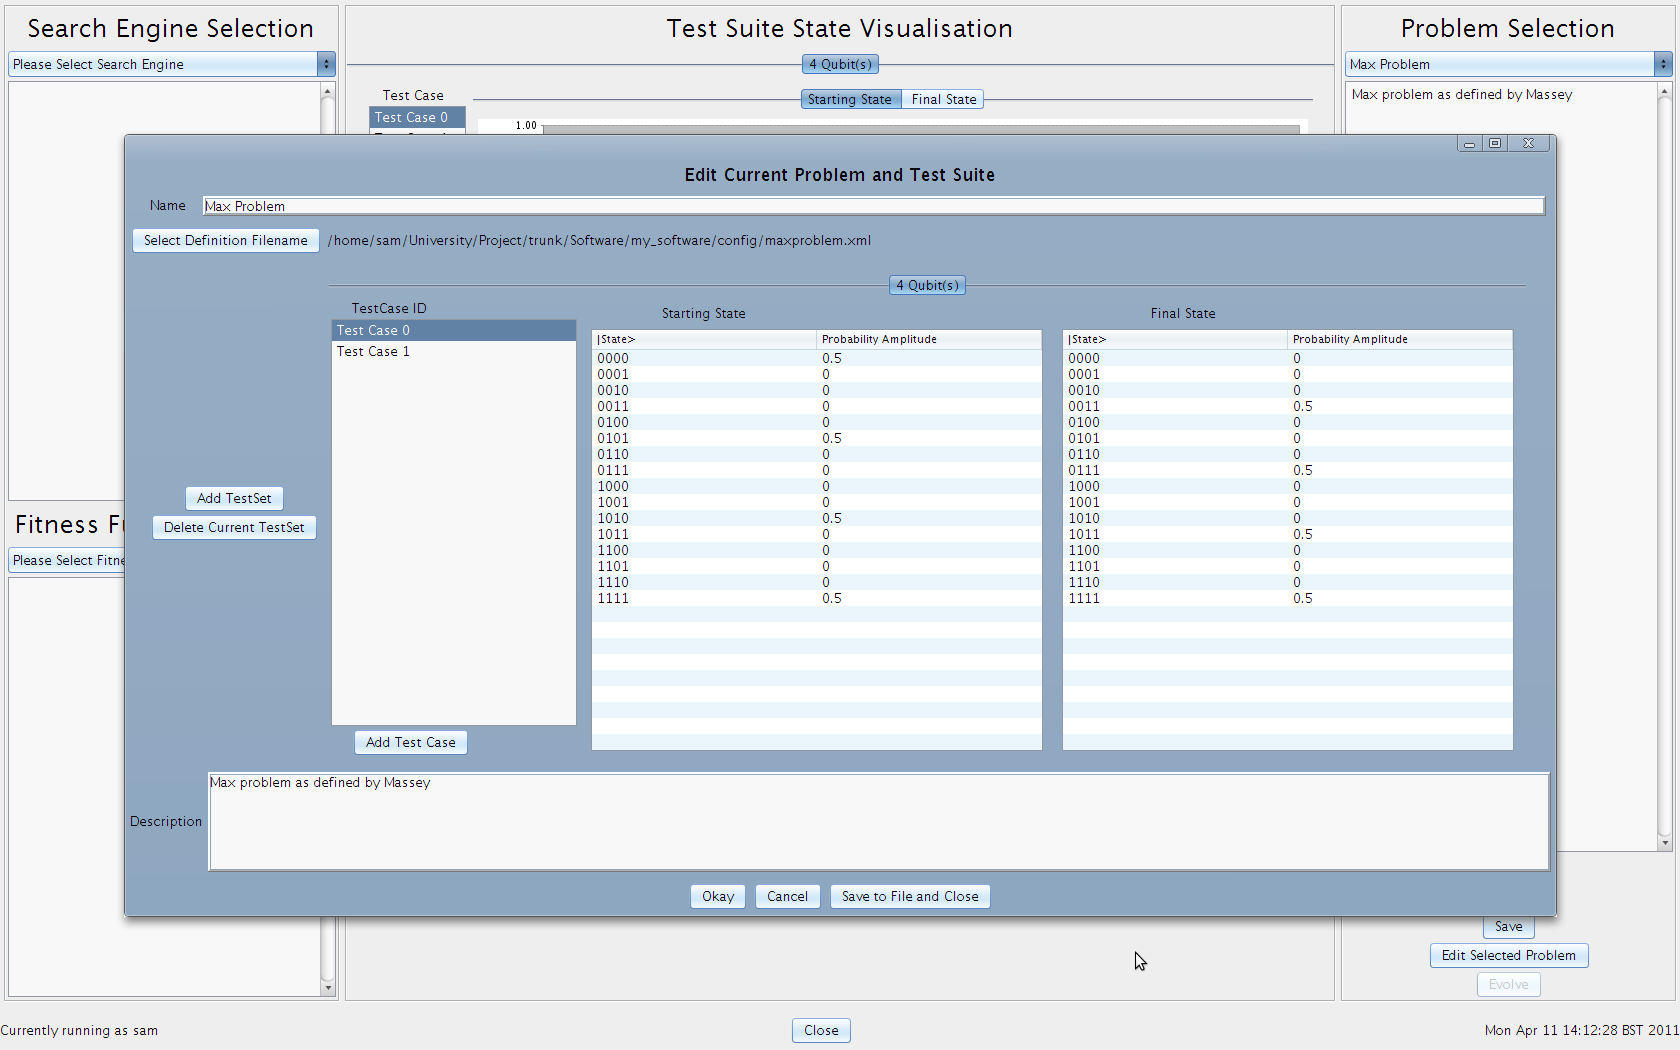
\includegraphics[width=\textwidth]{walkthrough6.png}
 \caption{Edit Current Problem and Test Suite dialog box}
 \label{fig:walkthrough6}
\end{figure}

\begin{figure}
  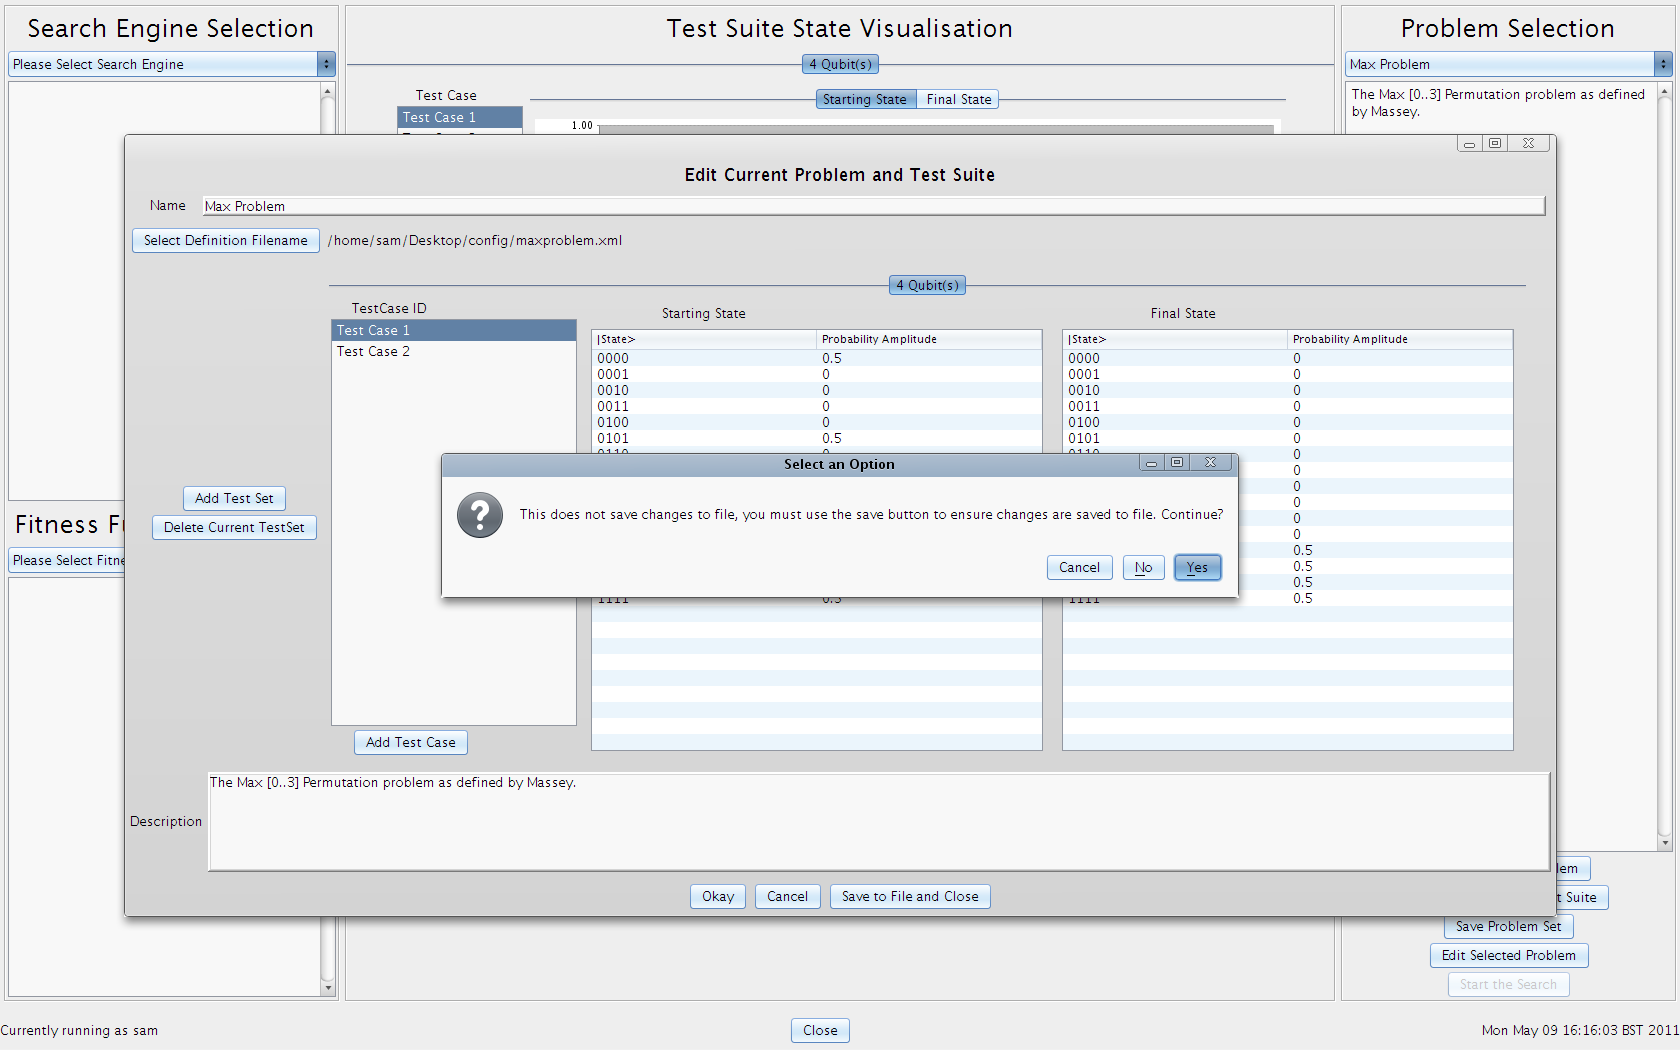
\includegraphics[width=\textwidth]{walkthrough7.png}
 \caption{Warning Produced by Pressing Okay}
 \label{fig:walkthrough7}
\end{figure}

\begin{figure}
  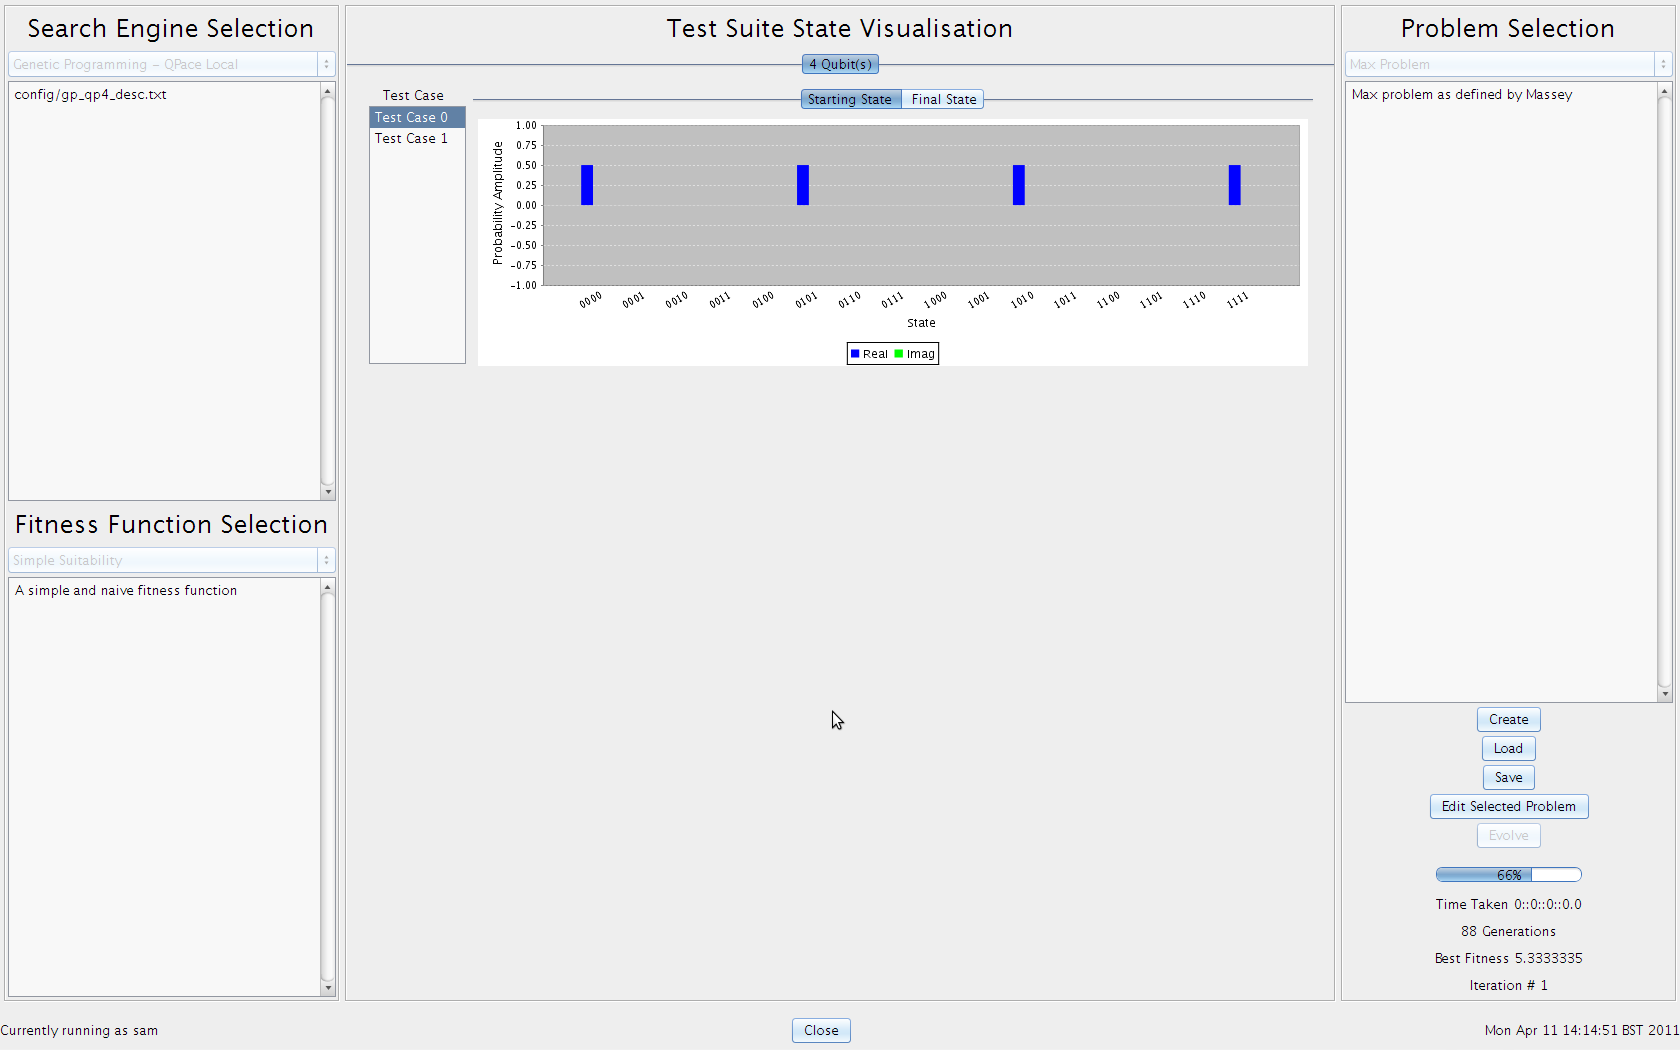
\includegraphics[width=\textwidth]{walkthrough8.png}
 \caption{Search Progress Statistics}
 \label{fig:walkthrough8}
\end{figure}

\begin{figure}
  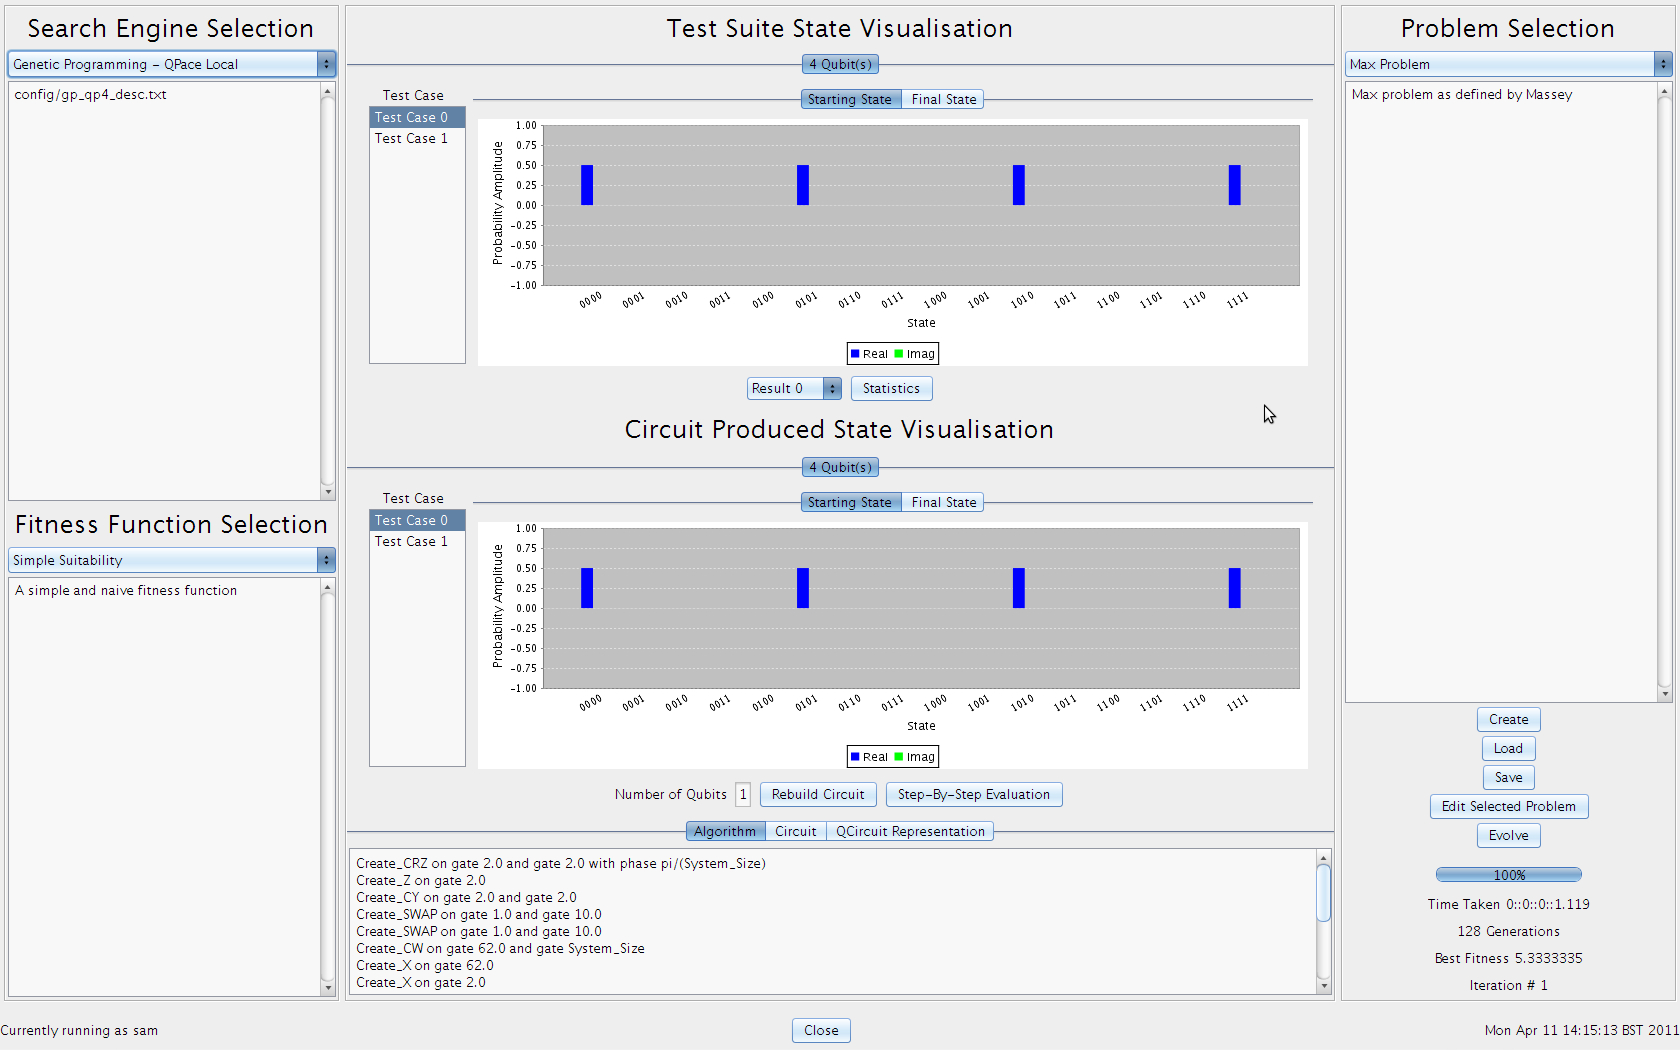
\includegraphics[width=\textwidth]{walkthrough9.png}
 \caption{Client GUI after Search is Complete}
 \label{fig:walkthrough9}
\end{figure}

\chapter{Experiment Data}

\section{Deutsch Experiment}
\label{sec:DeutschExpApp}
\subsection{Full Algorithm}
\label{sec:DeutschExpAppFullAlg}

\begin{algorithm}
 \begin{algorithmic}
\STATE Create\_Custom1 on gate Loop\_Vars[54.0]
\STATE Create\_H on gate Loop\_Vars[5.0]
\STATE Create\_CCustom1 on gate 1.0 and gate System\_Size
\STATE Create\_H on gate 1.0
\STATE Create\_V on gate 54.0
\STATE Create\_CCustom1 on gate 1.0 and gate System\_Size
\STATE Create\_H on gate 1.0
\STATE Create\_CX on gate 54.0 and gate 1.0
 \end{algorithmic}
\caption{Evolved Solution for Deutsch Problem}
\label{alg:evodeutsch}
\end{algorithm}








\clearpage
\section{Deutsch Jozsa Experiment}
\label{sec:deutschjozsa}

\begin{figure}[h!]
\centering
\subfigure[$f_1$]{
$
\begin{pmatrix}
1 & 0 & 0 & 0 & 0 & 0 & 0 & 0 \\
0 & 1 & 0 & 0 & 0 & 0 & 0 & 0\\
0 & 0 & 1 & 0 & 0 & 0 & 0 & 0\\
0 & 0 & 0 & 1 & 0 & 0 & 0 & 0\\
0 & 0 & 0 & 0 & 1 & 0 & 0 & 0\\
0 & 0 & 0 & 0 & 0 & 1 & 0 & 0\\
0 & 0 & 0 & 0 & 0 & 0 & 1 & 0\\
0 & 0 & 0 & 0 & 0 & 0 & 0 & 1
\end{pmatrix}
$
}
\subfigure[$f_2$]{
$
\begin{pmatrix}
0 & 0 & 0 & 0 & 1 & 0 & 0 & 0 \\
0 & 0 & 0 & 0 & 0 & 1 & 0 & 0\\
0 & 0 & 0 & 0 & 0 & 0 & 1 & 0\\
0 & 0 & 0 & 0 & 0 & 0 & 0 & 1\\
1 & 0 & 0 & 0 & 0 & 0 & 0 & 0\\
0 & 1 & 0 & 0 & 0 & 0 & 0 & 0\\
0 & 0 & 1 & 0 & 0 & 0 & 0 & 0\\
0 & 0 & 0 & 1 & 0 & 0 & 0 & 0
\end{pmatrix}
$
}
\subfigure[$f_3$]{
$
\begin{pmatrix}
1 & 0 & 0 & 0 & 0 & 0 & 0 & 0 \\
0 & 1 & 0 & 0 & 0 & 0 & 0 & 0\\
0 & 0 & 0 & 0 & 0 & 0 & 1 & 0\\
0 & 0 & 0 & 0 & 0 & 0 & 0 & 1\\
0 & 0 & 0 & 0 & 1 & 0 & 0 & 0\\
0 & 0 & 0 & 0 & 0 & 1 & 0 & 0\\
0 & 0 & 1 & 0 & 0 & 0 & 0 & 0\\
0 & 0 & 0 & 1 & 0 & 0 & 0 & 0
\end{pmatrix}
$
}
\\
\subfigure[$f_4$]{
$
\begin{pmatrix}
1 & 0 & 0 & 0 & 0 & 0 & 0 & 0 \\
0 & 0 & 0 & 0 & 0 & 1 & 0 & 0\\
0 & 0 & 1 & 0 & 0 & 0 & 0 & 0\\
0 & 0 & 0 & 0 & 0 & 0 & 0 & 1\\
0 & 0 & 0 & 0 & 1 & 0 & 0 & 0\\
0 & 1 & 0 & 0 & 0 & 0 & 0 & 0\\
0 & 0 & 0 & 0 & 0 & 0 & 1 & 0\\
0 & 0 & 0 & 1 & 0 & 0 & 0 & 0
\end{pmatrix}
$
}
\subfigure[$f_5$]{
$
\begin{pmatrix}
0 & 0 & 0 & 0 & 1 & 0 & 0 & 0 \\
0 & 1 & 0 & 0 & 0 & 0 & 0 & 0\\
0 & 0 & 1 & 0 & 0 & 0 & 0 & 0\\
0 & 0 & 0 & 0 & 0 & 0 & 0 & 1\\
1 & 0 & 0 & 0 & 0 & 0 & 0 & 0\\
0 & 0 & 0 & 0 & 0 & 1 & 0 & 0\\
0 & 0 & 0 & 0 & 0 & 0 & 1 & 0\\
0 & 0 & 0 & 1 & 0 & 0 & 0 & 0
\end{pmatrix}
$
}
\subfigure[$f_6$]{
$
\begin{pmatrix}
1 & 0 & 0 & 0 & 0 & 0 & 0 & 0 \\
0 & 0 & 0 & 0 & 0 & 1 & 0 & 0\\
0 & 0 & 0 & 0 & 0 & 0 & 1 & 0\\
0 & 0 & 0 & 1 & 0 & 0 & 0 & 0\\
0 & 0 & 0 & 0 & 1 & 0 & 0 & 0\\
0 & 1 & 0 & 0 & 0 & 0 & 0 & 0\\
0 & 0 & 1 & 0 & 0 & 0 & 0 & 0\\
0 & 0 & 0 & 0 & 0 & 0 & 0 & 1
\end{pmatrix}
$
}
\\
\subfigure[$f_7$]{
$
\begin{pmatrix}
0 & 0 & 0 & 0 & 1 & 0 & 0 & 0 \\
0 & 1 & 0 & 0 & 0 & 0 & 0 & 0\\
0 & 0 & 0 & 0 & 0 & 0 & 1 & 0\\
0 & 0 & 0 & 1 & 0 & 0 & 0 & 0\\
1 & 0 & 0 & 0 & 0 & 0 & 0 & 0\\
0 & 0 & 0 & 0 & 0 & 1 & 0 & 0\\
0 & 0 & 1 & 0 & 0 & 0 & 0 & 0\\
0 & 0 & 0 & 0 & 0 & 0 & 0 & 1
\end{pmatrix}
$
}
\subfigure[$f_8$]{
$
\begin{pmatrix}
0 & 0 & 0 & 0 & 1 & 0 & 0 & 0 \\
0 & 0 & 0 & 0 & 0 & 1 & 0 & 0\\
0 & 0 & 1 & 0 & 0 & 0 & 0 & 0\\
0 & 0 & 0 & 1 & 0 & 0 & 0 & 0\\
1 & 0 & 0 & 0 & 0 & 0 & 0 & 0\\
0 & 1 & 0 & 0 & 0 & 0 & 0 & 0\\
0 & 0 & 0 & 0 & 0 & 0 & 1 & 0\\
0 & 0 & 0 & 0 & 0 & 0 & 0 & 1
\end{pmatrix}
$
}
\caption{Matricies of Custom Gates Implementing the Eight Possible Functions}
 \label{fig:deutschjozsafunctions}
\end{figure}

\clearpage
\subsection{Search Parameters}
\label{sec:deutschjozsasearchparams}

\begin{figure}[h!]
\begin{center}
 \begin{tabular}{|cc|cc|}
\hline
  Population Size & 128 & Generations & 300 \\
  \# of Breeder Threads & 8 & \# of Evaluation Threads & 8 \\
  \# of Elites & 1 & Number of Iterations & 1 \\
  Minimum Initial Tree Depth & 10 & Maximum Initial Tree Depth & 20 \\
  CrossOver Rate & 0.9 & Mutation Rate & 0.0033846154 \\
\hline
 \end{tabular}
 \begin{tabular}{cc}
  \textbf{Search Engine} & Genetic Programming - QPace Local \\
  \textbf{Suitability Measure} & Simple Suitability - Non-Zero Count \\
 \end{tabular}
\begin{tabular}{|ccccccc|}
\hline
  Create\_H & Create\_X& Create\_Y& Create\_Z & Create\_R & Create\_Custom1 & Body \\
  Create\_CH & Create\_CX & Create\_CY & Create\_CZ & Create\_CR & Create\_CCustom1 & Iterate \\
   & Create\_CCX &  & &  &  &  \\
\hline
 \end{tabular}
\end{center}
\caption{Search Parameters used for Deutsch Jozsa Search}
\label{fig:deutschjozsaparams}
\end{figure}

\subsection{Full Algorithm}
\label{sec:DeutschJozsaExpAppFullAlg}

\begin{algorithm}
 \begin{algorithmic}
\STATE Create\_CR on gate 2.0 and gate 6.0 with phase 1.0
\STATE Create\_H on gate 2.0
\STATE Create\_H on gate 3.0
\STATE Create\_H on gate 1.0
\STATE Create\_Custom1 on gate 1.0
\STATE Create\_CR on gate Loop\_Vars[3.0] and gate 48.0 with phase Loop\_Vars[2.0]
\STATE Create\_CR on gate 2.0 and gate 6.0 with phase 1.0
\STATE Create\_H on gate 39.0
\STATE Create\_CR on gate 2.0 and gate 6.0 with phase 1.0
\STATE Create\_H on gate 2.0
\STATE Create\_H on gate 3.0
\STATE Create\_H on gate 31.0
\STATE Create\_CR on gate 2.0 and gate 6.0 with phase 1.0
\STATE Create\_H on gate Loop\_Vars[2.0]
\STATE Create\_H on gate 1.0
\STATE Create\_CR on gate 79.0 and gate Loop\_Vars[10.0] with phase Loop\_Vars[2.0]
 \end{algorithmic}
\caption{Evolved Solution for Deutsch Jozsa Problem}
\label{alg:evodeutschjozsa}
\end{algorithm}

\clearpage
\subsection{Full Circuits}
\label{sec:DeutschJozsaExpAppFullCirs}
\begin{figure}[h!]
\[
\Qcircuit @C=1.0em @R=.7em {
&\gate{H}&\qw&\qw&\qw&\\%2
&\qw&\gate{H}&\gate{C0}&\gate{H}&\\%1
}
\]
\caption{Deutsch Jozsa Solution - Two Qubits }
\end{figure}
\begin{figure}[h!]
\[
\Qcircuit @C=1.0em @R=.7em {
&\qw&\gate{H}&\qw&\qw&\qw&\qw&\\%3
&\gate{H}&\qw&\qw&\qw&\gate{H}&\qw&\\%2
&\qw&\qw&\gate{H}&\gate{C0}&\qw&\gate{H}&\\%1
}
\]
\caption{Deutsch Jozsa Solution - Three Qubits }
\end{figure}
\begin{figure}[h!]
\[
\Qcircuit @C=1.0em @R=.7em {
&\qw&\qw&\qw&\qw&\qw&\qw&\gate{H}&\qw&\\%4
&\qw&\gate{H}&\qw&\qw&\qw&\gate{H}&\qw&\qw&\\%3
&\gate{H}&\qw&\qw&\qw&\gate{H}&\qw&\qw&\qw&\\%2
&\qw&\qw&\gate{H}&\gate{C0}&\qw&\qw&\qw&\gate{H}&\\%1
}
\]
\caption{Deutsch Jozsa Solution - Four Qubits }
\label{fig:evodeutschjozsafourq}
\end{figure}

\clearpage
\section{0..3 Max Permutation Problem}
\label{sec:maxpermsol}

\subsection{Search Parameters}
\label{sec:maxpermsearchparams}

\begin{figure}[h!]
\begin{center}
 \begin{tabular}{|cc|cc|}
\hline
  Population Size & 128 & Generations & 128 \\
  \# of Breeder Threads & 8 & \# of Evaluation Threads & 8 \\
  \# of Elites & 1 & Number of Iterations & 1 \\
  Minimum Initial Tree Depth & 1 & Maximum Initial Tree Depth & 30 \\
  CrossOver Rate & 0.9 & Mutation Rate & 0.003846154 \\
\hline
 \end{tabular}
 \begin{tabular}{cc}
  \textbf{Search Engine} & Genetic Programming - QPace Local \\
  \textbf{Suitability Measure} & Simple Suitability - Zero Focessed \\
 \end{tabular}
 \begin{tabular}{|ccccc|}
\hline
  Create\_H & Create\_X & Create\_R & Body & Iterate \\
  Create\_CH & Create\_CX & Create\_CR & Create\_CCX & RevIterate \\
\hline
 \end{tabular}
\end{center}
\caption{Search Parameters Used for 0..3 Max Permutation Problem}
\label{fig:maxpermparams}
\end{figure}

\clearpage
\subsection{Algorithm}
\begin{algorithm}
 \begin{algorithmic}
\STATE \{
\STATE Iterate for 10.0 iterations \{
\STATE \}
\STATE \}
\STATE Create\_X on gate Loop\_Vars[8.0]
\STATE Create\_CX on gate 17.0 and gate 45.0
\STATE Create\_CH on gate 7.0 and gate 17.0
\STATE Iterate for 95.0 iterations \{
\STATE Create\_R on gate Loop\_Vars[4.0] with phase Loop\_Vars[1.0]
\STATE \}
\STATE Create\_H on gate 102.0
\STATE \{
\STATE \{
\STATE Create\_CCX on gate 2.0 and gate 1.0 with phase 2.0
\STATE \}
\STATE Create\_X on gate 2.0
\STATE \}
\STATE Iterate for 10.0 iterations \{
\STATE \}
\STATE Create\_CCX on gate System\_Size and gate 1.0 with phase 2.0
\end{algorithmic}
\caption{Full Algorithm to Produce the Solution for the Max Permutation Problem}
\label{alg:03permfullalg}
\end{algorithm}

\clearpage
\subsection{Measurement Probabilities}
\label{sec:maxpermmeasprobs}
\centering
 \begin{tabular}{c|c|c|c|c|}
\textbf{Test Case} & $\ket{00}$& $\ket{01}$& $\ket{10}$& $\ket{11}$ \\
1 & 0.25 & 0.00 & 0.25 & \textbf{0.50} \\
2 & 0.00 & 0.25 & \textbf{0.50} & 0.25 \\
3 & 0.25 & 0.00 & 0.25 & \textbf{0.50} \\
4 & 0.00 & 0.25 & \textbf{0.50} & 0.25 \\
5 & 0.25 & \textbf{0.50} & 0.25 & 0.00 \\
6 & 0.25 & \textbf{0.50} & 0.25 & 0.00 \\
7 & 0.25 & 0.00 & 0.25 & \textbf{0.50} \\
8 & 0.00 & 0.25 & \textbf{0.50} & 0.25 \\
9 & 0.25 & 0.00 & 0.25 & \textbf{0.50} \\
10 & 0.00 & 0.25 & \textbf{0.50} & 0.25 \\
11 & 0.25 & \textbf{0.50} & 0.25 & 0.00 \\
12 & 0.25 & \textbf{0.50} & 0.25 & 0.00 \\
13 & 0.25 & 0.00 & 0.25 & \textbf{0.50} \\
14 & 0.00 & 0.25 & \textbf{0.50} & 0.25 \\
15 & 0.25 & 0.00 & 0.25 & \textbf{0.50} \\
16 & 0.00 & 0.25 & \textbf{0.50} & 0.25 \\
17 & 0.25 & \textbf{0.50} & 0.25 & 0.00 \\
18 & 0.25 & \textbf{0.50} & 0.25 & 0.00 \\
19 & \textbf{0.50} & 0.25 & 0.00 & 0.25 \\
20 & \textbf{0.50} & 0.25 & 0.00 & 0.25 \\
21 & \textbf{0.50} & 0.25 & 0.00 & 0.25 \\
22 & \textbf{0.50} & 0.25 & 0.00 & 0.25 \\
23 & \textbf{0.50} & 0.25 & 0.00 & 0.25 \\
24 & \textbf{0.50} & 0.25 & 0.00 & 0.25
 \end{tabular}

The bold values are the probability of the desired states, the solution states.

\clearpage
\section{Quantum Fourier Transform Experiment}
\label{sec:quantfourtransexp}


\begin{figure}[h!]
\centering
\subfigure[Test Case $1$]{
$
\begin{pmatrix}
1 \\
0 \\
0 \\
0  
\end{pmatrix}
\rightarrow
\begin{pmatrix}
   0.50000 \\
   0.50000 \\
   0.50000 \\
   0.50000
\end{pmatrix}
$

}
\subfigure[Test Case $2$]{
$
\begin{pmatrix}
0 \\
1 \\
0 \\
0  
\end{pmatrix}
\rightarrow
\begin{pmatrix}
   0.50000 + 0.00000i \\
   0.00000 + 0.50000i \\
  -0.50000 + 0.00000i \\
  -0.00000 - 0.50000i  
\end{pmatrix}
$
}
\subfigure[Test Case $3$]{
$
\begin{pmatrix}
0 \\
0 \\
1 \\
0  
\end{pmatrix}
\rightarrow
\begin{pmatrix}
   0.50000 + 0.00000i \\
  -0.50000 + 0.00000i \\
   0.50000 - 0.00000i \\
  -0.50000 + 0.00000i 
\end{pmatrix}
$
}
\subfigure[Test Case $4$]{
$
\begin{pmatrix}
0 \\
0 \\
0 \\
1 
\end{pmatrix}
\rightarrow
\begin{pmatrix}
   0.50000 + 0.00000i \\
  -0.00000 - 0.50000i \\
  -0.50000 + 0.00000i \\
   0.00000 + 0.50000i 
\end{pmatrix}
$
}
\caption{Test Cases for Two Qubits}
 \label{fig:qfttwoqubits}
\end{figure}


\begin{figure}[h!]
\centering
\subfigure[Test Case $1$]{
$
\begin{pmatrix}
1 \\
0 \\
0 \\
0 \\
0 \\
0 \\
0 \\
0  
\end{pmatrix}
\rightarrow
\begin{pmatrix}
0.35355 + 0.00000i \\
0.35355 + 0.00000i \\
0.35355 + 0.00000i \\
0.35355 + 0.00000i \\
0.35355 + 0.00000i \\
0.35355 + 0.00000i \\
0.35355 + 0.00000i \\
0.35355 + 0.00000i
\end{pmatrix}
$

}
\subfigure[Test Case $2$]{
$
\begin{pmatrix}
0 \\
1 \\
0 \\
0 \\
0 \\
0 \\
0 \\
0  
\end{pmatrix}
\rightarrow
\begin{pmatrix}
0.35355 + 0.00000i \\
0.25000 + 0.25000i \\
0.00000 + 0.35355i \\
-0.25000 + 0.25000i \\
-0.35355 + 0.00000i \\
-0.25000 - 0.25000i \\
-0.00000 - 0.35355i \\
0.25000 - 0.25000i
\end{pmatrix}
$
}
\subfigure[Test Case $3$]{
$
\begin{pmatrix}
0 \\
0 \\
1 \\
0 \\
0 \\
0 \\
0 \\
0  
\end{pmatrix}
\rightarrow
\begin{pmatrix}
   0.35355 + 0.00000i \\
   0.00000 + 0.35355i \\
  -0.35355 + 0.00000i \\
  -0.00000 - 0.35355i \\
   0.35355 - 0.00000i \\
   0.00000 + 0.35355i \\
  -0.35355 + 0.00000i \\
  -0.00000 - 0.35355i
\end{pmatrix}
$
}
\subfigure[Test Case $4$]{
$
\begin{pmatrix}
0 \\
0 \\
0 \\
1 \\
0 \\
0 \\
0 \\
0
\end{pmatrix}
\rightarrow
\begin{pmatrix}
   0.35355 + 0.00000i \\
  -0.25000 + 0.25000i \\
  -0.00000 - 0.35355i \\
   0.25000 + 0.25000i \\
  -0.35355 + 0.00000i \\
   0.25000 - 0.25000i \\
   0.00000 + 0.35355i \\
  -0.25000 - 0.25000i
\end{pmatrix}
$
}
\subfigure[Test Case $5$]{
$
\begin{pmatrix}
0 \\
0 \\
0 \\
0 \\
1 \\
0 \\
0 \\
0
\end{pmatrix}
\rightarrow
\begin{pmatrix}
   0.35355 + 0.00000i \\
  -0.35355 + 0.00000i \\
   0.35355 - 0.00000i \\
  -0.35355 + 0.00000i \\
   0.35355 - 0.00000i \\
  -0.35355 + 0.00000i \\
   0.35355 - 0.00000i \\
  -0.35355 + 0.00000i
\end{pmatrix}
$
}
\subfigure[Test Case $6$]{
$
\begin{pmatrix}
0 \\
0 \\
0 \\
0 \\
0 \\
1 \\
0 \\
0
\end{pmatrix}
\rightarrow
\begin{pmatrix}
   0.35355 + 0.00000i \\
  -0.25000 - 0.25000i \\
   0.00000 + 0.35355i \\
   0.25000 - 0.25000i \\
  -0.35355 + 0.00000i \\
   0.25000 + 0.25000i \\
  -0.00000 - 0.35355i \\
  -0.25000 + 0.25000i
\end{pmatrix}
$
}
\subfigure[Test Case $7$]{
$
\begin{pmatrix}
0 \\
0 \\
0 \\
0 \\
0 \\
0 \\
1 \\
0
\end{pmatrix}
\rightarrow
\begin{pmatrix}
   0.35355 + 0.00000i \\
  -0.00000 - 0.35355i \\
  -0.35355 + 0.00000i \\
   0.00000 + 0.35355i \\
   0.35355 - 0.00000i \\
  -0.00000 - 0.35355i \\
  -0.35355 + 0.00000i \\
   0.00000 + 0.35355i
\end{pmatrix}
$
}
\subfigure[Test Case $8$]{
$
\begin{pmatrix}
0 \\
0 \\
0 \\
0 \\
0 \\
0 \\
0 \\
1
\end{pmatrix}
\rightarrow
\begin{pmatrix}
   0.35355 + 0.00000i \\
   0.25000 - 0.25000i \\
  -0.00000 - 0.35355i \\
  -0.25000 - 0.25000i \\
  -0.35355 + 0.00000i \\
  -0.25000 + 0.25000i \\
   0.00000 + 0.35355i \\
   0.25000 + 0.25000i
\end{pmatrix}
$
}
\caption{Test Cases for Two Qubits}
 \label{fig:qftthreequbits}
\end{figure}

\clearpage
\subsection{Search Parameters}
\label{sec:qftsearchparams}

\begin{figure}[h!]
\begin{center}
 \begin{tabular}{|cc|cc|}
\hline
  Population Size & 1280 & Generations & 1280 \\
  \# of Breeder Threads & 8 & \# of Evaluation Threads & 8 \\
  \# of Elites & 1 & Number of Iterations & 1 \\
  Minimum Initial Tree Depth & 10 & Maximum Initial Tree Depth & 20 \\
  CrossOver Rate & 0.9 & Mutation Rate & 0.003846154 \\
\hline
 \end{tabular}
 \begin{tabular}{cc}
  \textbf{Search Engine} & Genetic Programming - QPace Local \\
  \textbf{Suitability Measure} & Phase Sensitive \\
 \end{tabular}
 \begin{tabular}{|cccc|}
\hline
  Create\_H & Create\_R & Create\_SWAP & Body \\
  Create\_CH  & Create\_CR & Iterate & RevIterate\\
\hline
 \end{tabular}
\end{center}
\caption{Algorithm Instructions used for Quantum Fourier Transform Search}
\label{fig:qftparams}
\end{figure}


\clearpage
\subsection{Algorithm}
\label{sec:evoqftalgo}
\begin{algorithm}
 \begin{algorithmic}
\STATE Create\_SWAP on gate 4.0 and gate 1.0
\STATE Create\_CH on gate 1.0 and gate 5.0
\STATE Create\_SWAP on gate 5.0 and gate (Loop\_Vars[4.0])+(16.0)
\STATE Create\_CH on gate 1.0 and gate 5.0
\STATE Iterate for 5.0 iterations \{
\STATE Create\_CH on gate 1.0 and gate 6.0
\STATE \}
\STATE Create\_SWAP on gate 14.0 and gate 1.0
\STATE Create\_CR on gate (14.0)x(Loop\_Vars[30.0]) and gate Loop\_Vars[Loop\_Vars[5.0]] with phase Loop\_Vars[3.0]
\STATE Create\_CH on gate 1.0 and gate 5.0
\STATE Create\_CH on gate 1.0 and gate 5.0
\STATE Create\_CR on gate 20.0 and gate Loop\_Vars[Loop\_Vars[8.0]] with phase (Loop\_Vars[3.0])x(1.0)
\STATE Create\_CH on gate 5.0 and gate 5.0
\STATE Create\_SWAP on gate 20.0 and gate 5.0
\STATE Create\_CH on gate 1.0 and gate 6.0
\STATE Create\_SWAP on gate Loop\_Vars[(Loop\_Vars[38.0])-((80.0)x(Loop\_Vars[9.0]))] and gate 1.0
\STATE Create\_SWAP on gate 9.0 and gate 1.0
\STATE \{
\STATE Create\_CH on gate 1.0 and gate 5.0
\STATE Create\_H on gate 16.0
\STATE \}
\STATE Create\_SWAP on gate ((Loop\_Vars[16.0])-(Loop\_Vars[Loop\_Vars[9.0]]))-(14.0) and gate 16.0
\STATE Create\_H on gate 23.0
\STATE Create\_CH on gate 9.0 and gate 5.0
\STATE Create\_H on gate (Loop\_Vars[9.0])+(7.0)
\STATE Create\_SWAP on gate Loop\_Vars[9.0] and gate (Loop\_Vars[9.0])+(7.0)
\STATE Iterate for Loop\_Vars[9.0] iterations \{
\STATE Create\_CR on gate Loop\_Vars[Loop\_Vars[4.0]] and gate 20.0 with phase 3.0
\STATE Create\_CH on gate 1.0 and gate 5.0
\STATE Create\_SWAP on gate 4.0 and gate 1.0
\STATE Create\_H on gate 16.0
\STATE Create\_SWAP on gate 9.0 and gate 23.0
\STATE Create\_SWAP on gate Loop\_Vars[4.0] and gate 14.0
\STATE Create\_CR on gate 0.0 and gate (5.0)-(Loop\_Vars[4.0]) with phase 2.0
\STATE Create\_CH on gate 1.0 and gate 5.0
\STATE Create\_CR on gate 7.0 and gate 12.0 with phase Loop\_Vars[3.0]
\STATE Create\_H on gate 10.0
\STATE Create\_CH on gate 1.0 and gate 5.0
\STATE Create\_CR on gate 1.0 and gate Loop\_Vars[Loop\_Vars[9.0]] with phase Loop\_Vars[3.0]
\STATE Create\_H on gate Loop\_Vars[((Loop\_Vars[6.0])-((9.0)-((9.0)-(Loop\_Vars[Loop\_Vars[34.0]]))))-(-19.0)]
\STATE \}
 \end{algorithmic}
\caption{Full Algorithm to Produce the Quantum Fourier Transform}
\label{alg:qftfullalg}
\end{algorithm}


\clearpage
\subsection{Circuits}
\label{sec:evoqftcir}
\begin{figure}[h!]
\subfigure[Two Qubits]{
$
\Qcircuit @C=1.0em @R=.7em {
&\qswap &\qw&\ctrl{1} &\gate{H}&\qw&\\%2
&\qswap \qwx &\gate{H}&\gate{R(2.0)} \qwx &\qw&\qw&\\%1
&&&
}
$
}
\subfigure[Three Qubits]{
$
\Qcircuit @C=1.0em @R=.7em {
&\qswap &\qw&\qw&\qw&\gate{R(2.0)}&\ctrl{2} &\gate{H}&\qw&\\%3
&\qw \qwx&\qw&\ctrl{1} &\gate{H}&\ctrl{-1} \qwx&\qw \qwx&\qw&\qw&\\%2
&\qswap \qwx &\gate{H}&\gate{R(2.0)} \qwx &\qw&\qw&\gate{R(3.0)} \qwx &\qw&\qw&\\%1
}
$
}
\subfigure[Four Qubits]{
$
\Qcircuit @C=1.0em @R=.7em {
&\qswap &\qw&\gate{R(2.0000)}&\qw&\qw&\gate{R(2.0000)}&\qw&\qw&\gate{R(2.0000)}&\ctrl{3} &\gate{H}&\qw&\\%4
&\qw \qwx&\qw&\ctrl{-1} \qwx&\qw&\qw&\qw \qwx&\ctrl{2} &\gate{H}&\qw \qwx&\qw \qwx&\qw&\qw&\\%3
&\qw \qwx&\qw&\qw&\ctrl{1} &\gate{H}&\ctrl{-2} \qwx&\qw \qwx&\qw&\qw \qwx&\qw \qwx&\qw&\qw&\\%2
&\qswap \qwx &\gate{H}&\qw&\gate{R(2.0000)} \qwx &\qw&\qw&\gate{R(3.0000)} \qwx &\qw&\ctrl{-3} \qwx&\gate{R(4.0000)} \qwx &\qw&\qw&\\%1
}
$
\label{fig:appevoqft4qubits}
}
\caption{Evolved Quantum Fourier Transform Solution}
\label{fig:appevoqftsol}
\end{figure}
\chapter{Suitability Measure Definitions}
\label{sec:suitmeasdefs}
All suitability measures are defined using the polar form $re^{i\theta}$.
Subscript F indicates the Final state produced by the circuit generated from the algorithm under evaluation.
Subscript E indicated the Expected final state as defined in the current test case.
$N$ is the system size.

\begin{equation}
 \delta(a,b)=
\left\{
  \begin{array}{cc} 1, & \mbox{if } |a-b|<ACCURACY\\ 
  0, & \mbox{otherwise}\end{array}
\right.
\end{equation}
\begin{equation}
 \delta(a,b,c,d)=
\left\{
  \begin{array}{cc} 1, & \mbox{if } |a-b|<ACCURACY\wedge|c-d|<ACCURACY\\ 
  0, & \mbox{otherwise}\end{array}
\right.
\end{equation}


\section{Simple Suitability Measure}
$ACCURACY=10^{-8}$
\begin{equation}
 fitness=\sum_{i=0}^{2^N-1}|{r_F}_i-{r_E}_i|
\end{equation}

\begin{equation}
 hits=\sum_{i=0}^{2^N-1}\delta({r_F}_i,{r_E}_i)
\end{equation}


\section{Phase Aware Suitability Measure}
$ACCURACY=10^{-8}$
\begin{equation}
 fitness=\sum_{i=0}^{2^N-1}|{r_F}_i-{r_E}_i|+|{\theta_F}_i-{\theta_E}_i|
\end{equation}

\begin{equation}
 hits=\sum_{i=0}^{2^N-1}\delta({r_F}_i,{r_E}_i,{\theta_F}_i,{\theta_E}_i)
\end{equation}


\chapter{Full Requirements}
\label{sec:reqs}
\section{Framework}
\section{Fully Functional Tool}
\section{Client and GUI}
\cleardoublepage
\begingroup
\advance\textwidth\pdfpagewidth
\hsize=\textwidth\linewidth=\hsize\columnwidth=\hsize
\pdfpagewidth=2\pdfpagewidth

\chapter{Architechture Diagram}
\label{sec:archdesign}
\centering
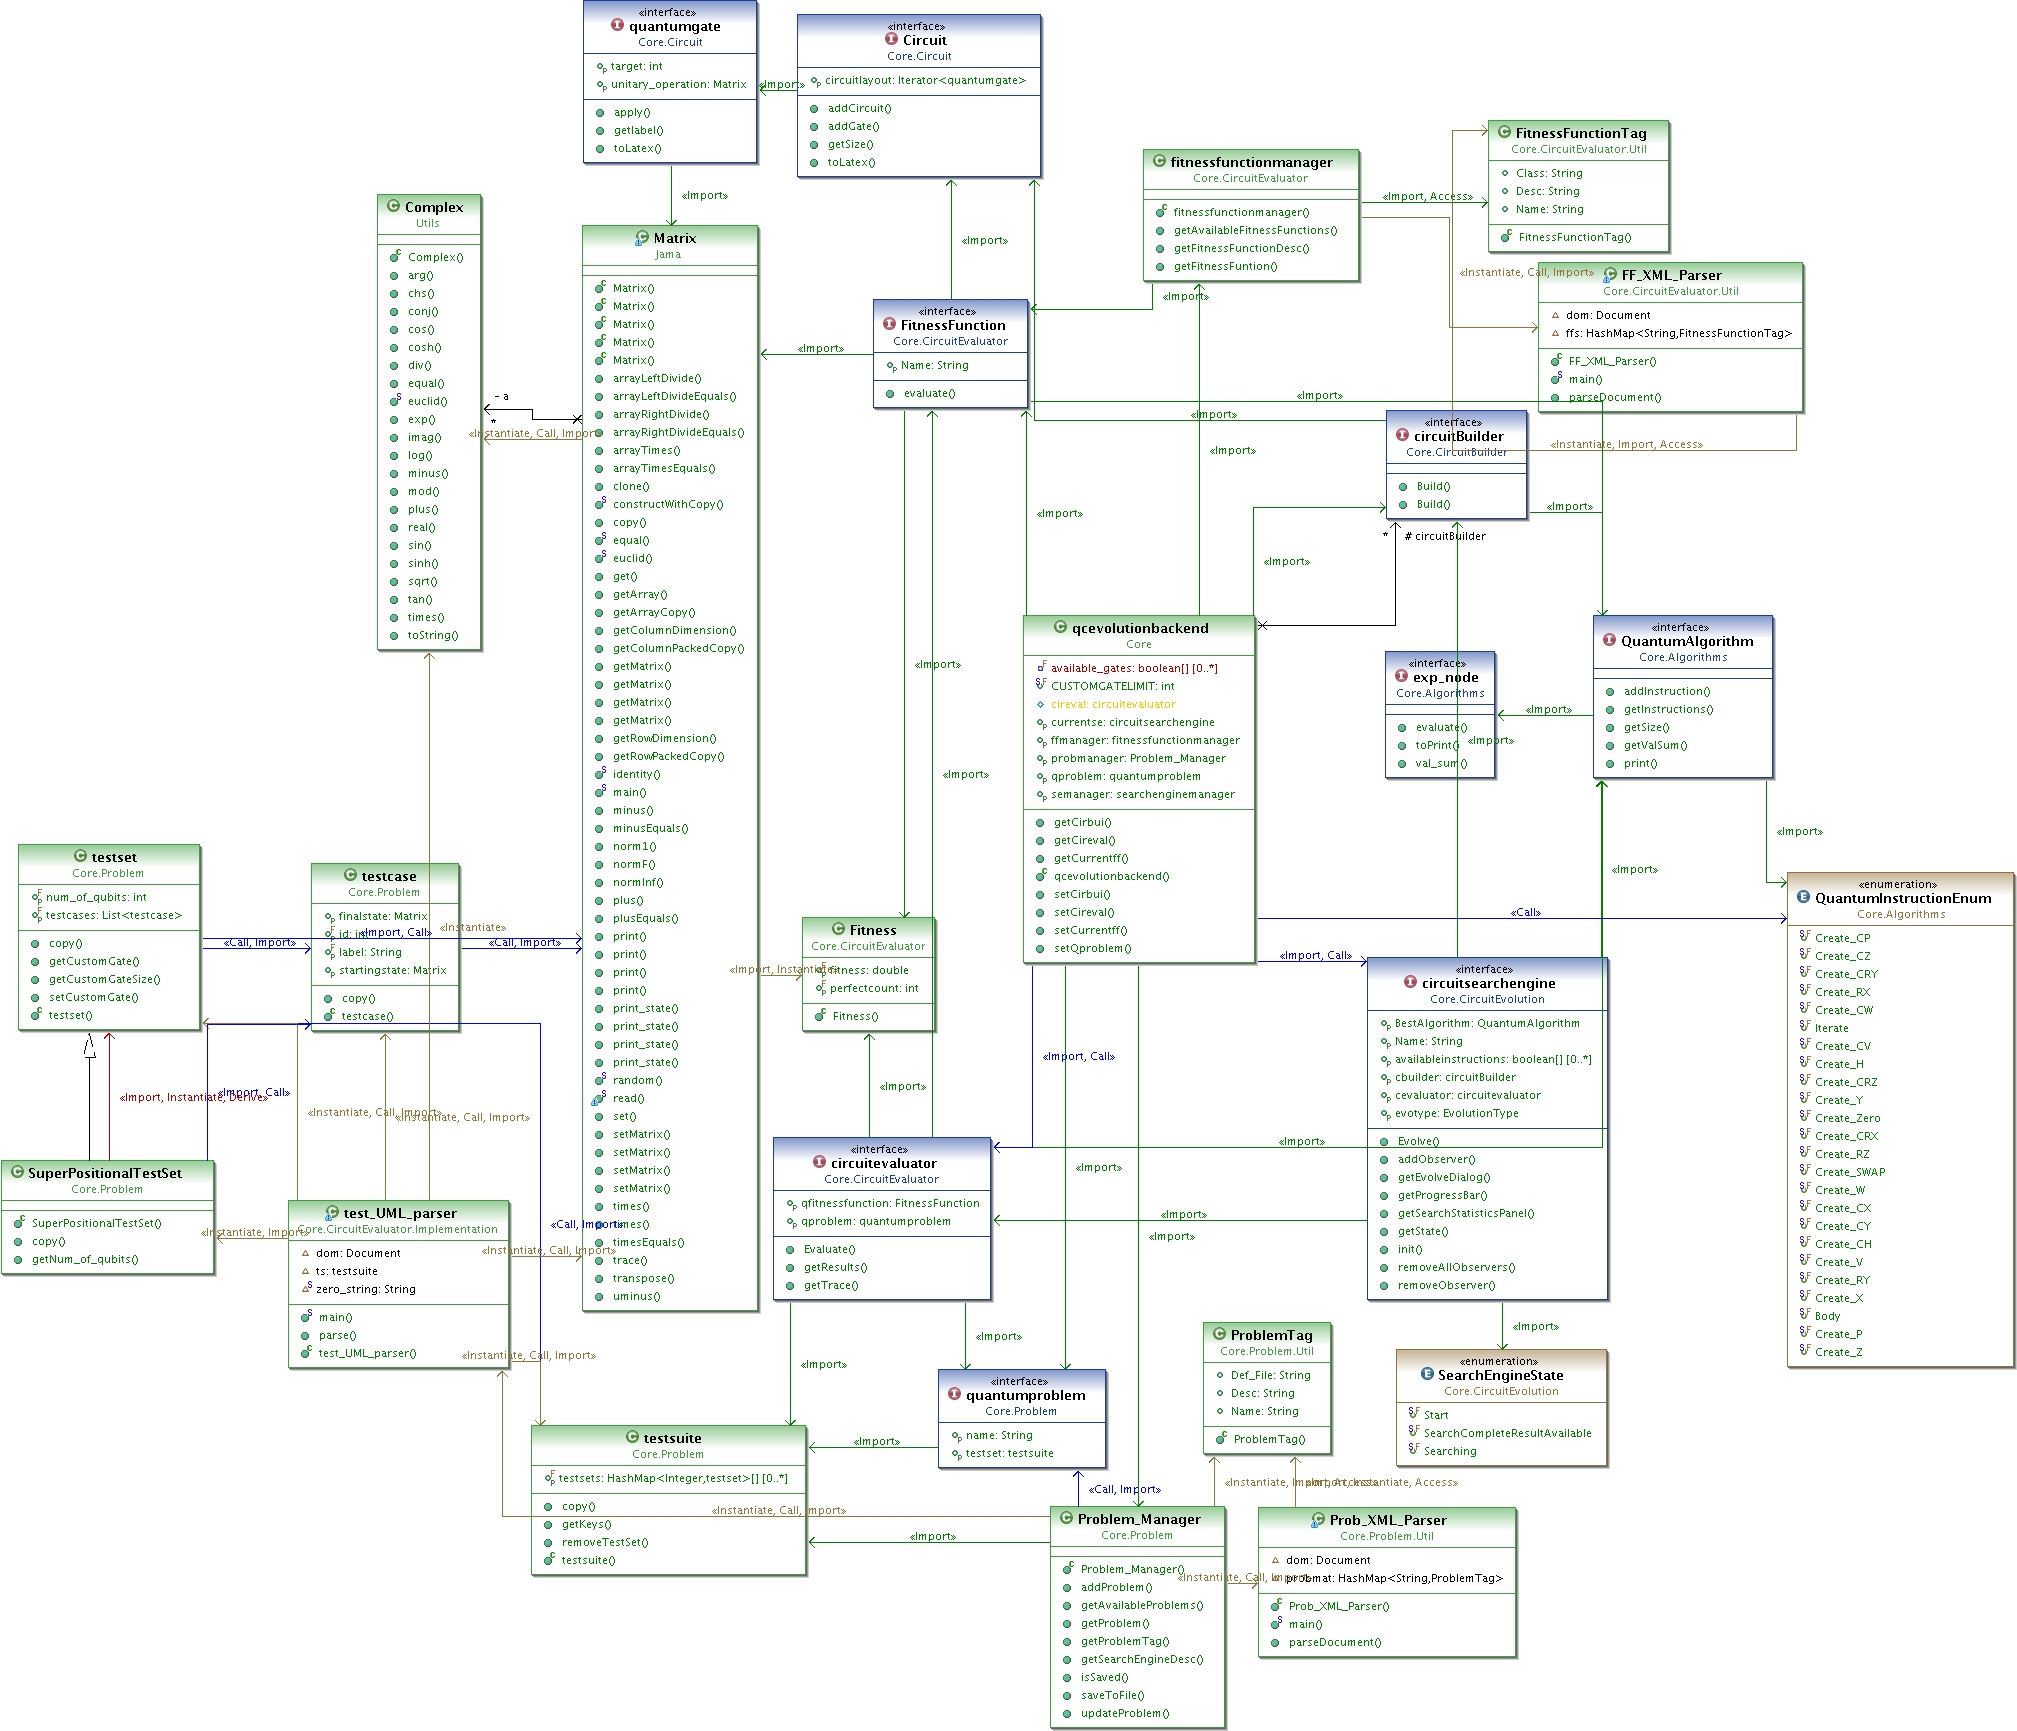
\includegraphics[height=0.85\textheight]{highlevelarchitecture.jpg}
\cleardoublepage
\endgroup

\chapter{XML Outlines}
\section{Search Engine XML Outline}
\label{sec:semanspecxml}
\lstset{language = XML}
\begin{lstlisting}
 <searchengine>
	<se>
	  <Name>SEARCH ENGINE NAMES</Name>
	  <Class>IMPLEMENTING FULLY QUALIFIED CLASS NAME</Class>
	  <Desc>SEARCH ENGINE DESCRIPTION</Desc>
	</se>
</searchengine>
\end{lstlisting}

\section{Problem Definition XML Outline}
\label{sec:probmanspecxml}
\lstset{language = XML}
\begin{lstlisting}
<Problems>
	<prob>
	  <Name>PROBLEM NAME</Name>
	  <DefFile>PROBLEM DEFINITION FILE</DefFile>
	  <Desc>PROBLEM DESCRIPTION</Desc>
	</prob>
</Problems>
\end{lstlisting}

\clearpage
\begin{landscape}

\chapter{Available Algorithm Instructions}
\label{sec:alginstructionlist}
\centering
\begin{tabular}{|c|c|c|c|c|}
\hline
\textbf{Instruction} & \textbf{Action} & & \textbf{Instruction} & \textbf{Action}  \\
\hline
\textbf{Create\_H} & Create a Hadamard Gate & & \textbf{Create\_CH} & Create a Controlled Hadamard Gate \\
\hline
\textbf{Create\_X} & Create a Pauli-X Gate & & \textbf{Create\_CX} & Create a Controlled Pauli-X Gate \\
\hline
\textbf{Create\_Y} & Create a Pauli-Y Gate & & \textbf{Create\_CY} & Create a Controlled Pauli-Y Gate \\
\hline
\textbf{Create\_Z} & Create a Pauli-Z Gate & & \textbf{Create\_CZ} & Create a Controlled Pauli-Z Gate \\
\hline
\textbf{Create\_P} & Create a Phase Gate & & \textbf{Create\_CP} & Create a Controlled Phase Gate \\
\hline
\textbf{Create\_V} & Create a V Gate & & \textbf{Create\_CV} & Create a Controlled V Gate \\
\hline
\textbf{Create\_W} & Create a W Gate & & \textbf{Create\_CW} & Create a Controlled W Gate \\
\hline
\textbf{Create\_RX} & Create a Rotate-X Gate & & \textbf{Create\_CRX} & Create a Controlled Rotate-X Gate \\
\hline
\textbf{Create\_RY} & Create a Rotate-Y Gate & & \textbf{Create\_CRY} & Create a Controlled Rotate-Y Gate \\
\hline
\textbf{Create\_RZ} & Create a Rotate-Z Gate & & \textbf{Create\_CRZ} & Create a Controlled Rotate-Z Gate \\
\hline
\textbf{Create\_SWAP} & Create a SWAP Gate & &  &  \\
\hline
\textbf{Iterate} & Run Sub-Algorithm$[0]$ for $n$ iterations & & \textbf{RevIterate} & Run Sub-Algorithm$[0]$ for $n$ iterations in reverse order\\
\hline
\textbf{Body} & Perform each Sub-Algorithm in turn & & & \\
\hline
\textbf{Create\_Custom1} & Create Custom Gate Number $1$ & & \textbf{Create\_CCustom1} & Create a Controlled Custom Gate Number $1$ \\
\hline
\textbf{Create\_Custom2} & Create Custom Gate Number $2$ & & \textbf{Create\_CCustom2} & Create a Controlled Custom Gate Number $2$ \\
\hline
\textbf{Create\_Custom3} & Create Custom Gate Number $3$ & & \textbf{Create\_CCustom3} & Create a Controlled Custom Gate Number $3$ \\
\hline
\end{tabular}
\clearpage
\end{landscape}